\chapter{Reconstruction expérimentale d'événements \ttbar} \label{chap:mtt_reco}

Les \cref{chap:zprime,chap:higgs} sont consacrés à la recherche de nouvelle physique dans le spectre de masse invariante de paires \ttbar. Avant de pouvoir chercher de quelconques déviations dans le spectre de masse, il faut être capable de reconstruire la masse invariante du système \ttbar. Ce chapitre présente les techniques mises en œuvre pour la reconstruction de la masse invariante de paires \ttbar.

\section{Masse invariante du système \ttbar}

En utilisant le quadrivecteur énergie-impulsion ($p = \left(E,\,\vec{p}\right)$), la masse invariante est définie comme la norme de $p$ :
\begin{align*}
  m^2 &= \norm{p}^2 = E^2 - \norm{\vec{p}}^2
\end{align*}

Concentrons nous uniquement sur la désintégration semi-leptonique de paires \ttbar, c'est-à-dire un quark top qui se désintègrent en \Plepton{}\Pneutrino{}\Pbottom, et le deuxième en \Pbottom{}\Pquark{}\APquark (voir \cref{fig:top_pair_decay_semileptonic})\footnote{Ce choix particulier sera expliqué en détail dans le chapitre suivant.}. Toutes les particules peuvent être reconstruites, excepté le neutrino. En effet, n'interagissant que très faiblement avec la matière, les neutrinos traversent le détecteur sans laisser de dépôts dans les sous-détecteurs. Le seul moyen d'identifier les neutrinos est d'utiliser l'énergie transverse manquante. En faisant le bilan d'énergie de la collision dans le plan transverse, le neutrino apparait comme de l'énergie manquante. Dans le cas d'une désintégration \ttbar, on identifie la totalité de l'énergie transverse manquante comme venant du neutrino.

Afin de reconstruire la masse invariante du système \ttbar, il faut être capable de reconstruire la cinématique de chaque produit de la désintégration. On peut ensuite reconstruire la masse invariante \ttbar :
\begin{align} \label{eq:invariant_mass_tt}
  m_{\ttbar} &= \norm{ p_{\Plepton} + p_{\Pneutrino} + p_{\Pquark} + p_{\APquark} + p_{\Pbottom}^{\text{hadronique}} + p_{\Pbottom}^\text{leptonique} }
\end{align}

Deux problèmes majeurs se posent :
\begin{itemize}
    \item 4 jets composent l'état final d'une désintégration \ttbar. Il faut donc être capable de correctement identifier ces jets parmi les nombreux jets de \pu ou de radiations dans l'événement. Pour cela, diverses techniques peuvent être employées, décrites plus loin dans ce chapitre.
    \item L'énergie transverse manquante est utilisée pour reconstruire le neutrino. Comme le bilan d'énergie ne peut être effectué que dans le plan transverse, seule l'impulsion transverse du neutrino est définie, c'est-à-dire $p_x^{\Pnu}$ et $p_y^{\Pnu}$. Il faut donc trouver un moyen de reconstruire $p_z^{\Pnu}$ qui sera utilisé dans le calcul de la masse invariante \ttbar. C'est l'objet de la \cref{sec:neutrino}.
\end{itemize}

Une fois ces problèmes surmontés, il est possible de reconstruire la masse invariante pour chaque événement.

\section{Reconstruction du neutrino} \label{sec:neutrino}

Comme on a vu précédemment, la présence d'un neutrino se caractérise par de l'énergie manquante. En considérant que la seule source d'énergie manquante dans l'événement provient du neutrino, on a alors
\begin{align*}
  p_t^{\Pneutrino} &= \met
\end{align*}

Afin de reconstruire la masse invariante, il faut pouvoir reconstruire la composante longitudinale de l'impulsion transverse du neutrino. On sait que le neutrino émis vient obligatoirement de la désintégration d'un boson \PW en $\Plepton + \Pneutrino$. On peut déterminer la composante $p_z$ de l'impulsion du neutrino en utilisant comme contrainte la valeur de la masse du boson \PW ($m = \SI{80.385 \pm 0.015}{\GeV}$ \citep{pdg}). On a :
\begin{align*}
  m_{\PW}^2 &= \left( E_{\Pneutrino} + E_{\Plepton} \right)^2 - \norm{ \vec{p}_{\Pneutrino} + \vec{p}_{\Plepton} }^2 \\
  &= m_{\Plepton} + 2E_{\Pneutrino}E_{\Plepton} - 2 \vec{p}_{\Pneutrino} \cdot \vec{p}_{\Plepton}
\end{align*}

Après quelques calculs, on obtient une équation d'ordre 2 permettant de déterminer $p_z^{\Pnu}$ :
\begin{align*}
  a \, \left( p_z^{{\Pneutrino}} \right)^2 + b \, p_z^{{\Pneutrino}} + c &= 0
\end{align*}
avec
\begin{align*}
  a &= E_{\Plepton}^2 - \left( p_z^{{\Plepton}} \right)^2 \\
  b &= \left( m_{\Plepton}^2 - m_{\PW}^2 - 2 \left( p_x^{\Plepton} p_x^{\Pneutrino} + p_y^{\Plepton} p_y^{\Pneutrino} \right) \right) p_z^{\Plepton} \\
  c &= E_{\Plepton}^2 \left( p_z^{\Plepton} \right)^2 - \left( \frac{1}{2} \left( m_{\PW}^2 - m_{\Plepton}^2 \right) + p_x^{\Plepton} p_x^{\Pneutrino} + p_y^{\Plepton} p_y^{\Pneutrino} \right)^2
\end{align*}

\begin{figure}[tbp]
    \centering
    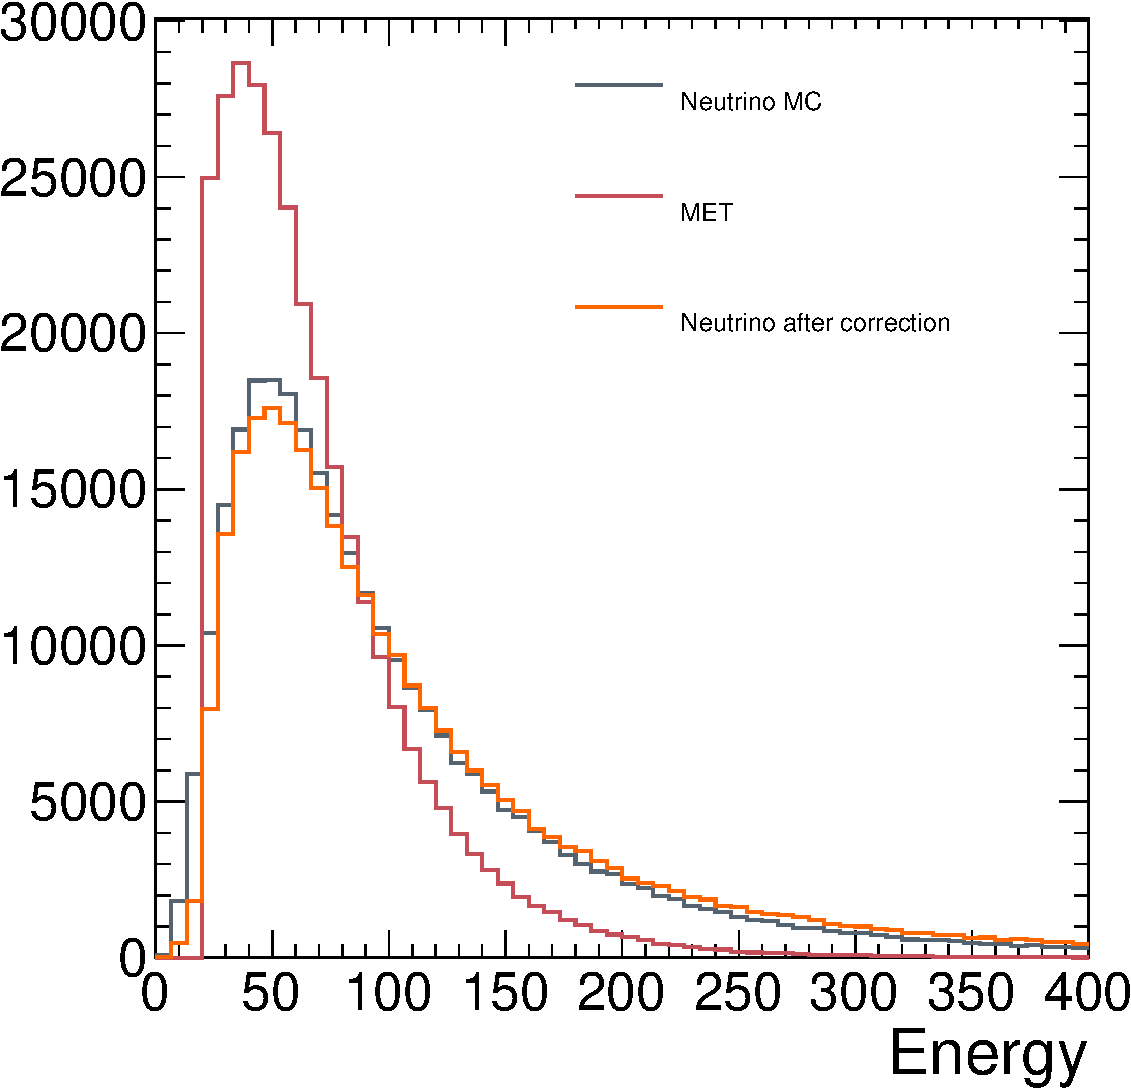
\includegraphics[width=0.55\textwidth]{chapitre6/figs/neutrino_energy/plot_met_energy.pdf}
    \caption{Effet de la reconstruction de la composante longitudinale du neutrino sur la mesure de l'énergie du neutrino sur des événements \ttbar simulés (en \textcolor{rouge_grandmere}{rouge}, avant reconstruction de $p_z$, en \textcolor{orange}{orange} après reconstruction). À titre de comparaison, l'énergie du neutrino au niveau générateur (en \textcolor{bleu_gris}{gris}) est aussi tracée.}
    \label{fig:neutrino_correction}
\end{figure}

Dans \tilde\SI{16}{\%} des cas, cette équation n'a pas de solution réelle. Cela peut être le cas lorsque l'énergie transverse manquante est surestimée. Dans ce cas, on cherche une solution réelle en faisant varier $p_x^{\Pneutrino}$ et $p_y^{\Pneutrino}$ de façon identique et synchronisée jusqu'à obtenir une solution réelle.

Lorsque l'on obtient deux solutions réelles, le choix est fait en utilisant la contrainte de la masse du quark top. Le neutrino provient en effet de la cascade de désintégration $\Ptop \rightarrow \Pbottom \PW$, $\PW \rightarrow \Plepton \Pneutrino$. On retient la solution qui donne la masse invariante à trois corps entre le lepton, le neutrino et le jet \Pbottom provenant de la désintégration leptonique d'un quark top\footnote{Le choix de ce jet est l'objet de la \cref{sec:chi2}} la plus proche de la masse du quark top.

\medskip

La \cref{fig:neutrino_correction} présente l'effet de la reconstruction de la composante longitudinale sur la mesure de l'énergie du neutrino. Avant reconstruction, l'énergie du neutrino est clairement sous estimée. Une fois $p_z^{\Pnu}$ reconstruit, l'énergie du neutrino coïncide avec l'énergie du neutrino générée. On mesure ici toute l'importance de la reconstruction du neutrino sur la mesure de l'énergie, et donc sur la reconstruction de la masse invariante du système \ttbar.

\section{Choix de la bonne combinaison de jets} \label{sec:chi2}

Lors d'une désintégration \ttbar dans le canal semi-leptonique, 4 jets composent l'état final : 2 jets de \Pbottom, provenant de la désintégrations des deux quarks top, et deux jets de quark légers, provenant de la désintégration hadronique d'un des bosons \PW.

De nombreux jets additionnels sont produits lors d'une collision au LHC, venant du \pu, de l'événement sous-jacent, de radiations de gluon, etc. Il faut donc un moyen d'identifier précisément les jets provenant de la désintégration \ttbar parmi tous les jets de l'événement. Deux méthodes sont étudiées dans cette section, la méthode de tri par $\chi^2$, et la méthode de tri par MVA (\emph{Multi-Variate Analysis}, analyse multi-variée).

\medskip

Ces deux méthodes sont utilisées après sélection. Cette sélection sera détaillée dans les prochains chapitres, puisqu'elle est dépendante de l'analyse. Néanmoins, on sélectionne typiquement des événements ayant un seul lepton isolé (électron ou muon), et au moins 4 jets. Ces événements constituent la signature expérimentale d'un événement \ttbar, et sont appelés événements candidats \ttbar.

\subsection{Algorithme de tri par \texorpdfstring{$\chi^2$}{chi²}}

Pour chaque événement candidat \ttbar, parmi $N (\geq 4)$ jets sélectionnés, on distingue $\binom{N}{N - 4}$ sous-ensembles de 4 jets. Pour chaque sous ensemble, on compte 12 combinaisons possibles pour assigner les jets si l'on considère les jets provenant de la désintégration du \PW hadronique indiscernables.

\medskip

Afin de choisir la bonne combinaison, on minimise une variable de $\chi^2$, construite à partir de composantes qui permettent de discriminer entre les bonnes et les mauvaises combinaisons. Le $\chi^2$ total est donné par
\begin{align} \label{eq:chi2}
  \chi^2 &= \chi^2_{m_{\Ptop}^{\text{lept.}}} + \chi^2_{m_{\Ptop}^{\text{hadr.}}} + \chi^2_{m_{\PW}^{\text{hadr.}}} + \chi^2_{H_{T}^{\text{frac.}}}
\end{align}
où

\begin{align*}
  \chi^2_X &= \frac{\left( X_\text{mesuré} - \left\langle X_\text{MC} \right\rangle \right)^2}{\sigma_\text{MC}^2}
\end{align*}
avec $X$ le discriminant considéré, $X_\text{mesuré}$ la valeur mesurée de ce discriminant, $\left\langle X_\text{MC} \right\rangle$ la valeur de référence du discriminant et $\sigma_\text{MC}$ l'incertitude sur la valeur de référence du discriminant.

Les discriminants formant le $\chi^2$ total sont :
\begin{itemize}
    \item $\chi^2_{m_{\Ptop}^{\text{lept.}}}$ : masse du quark top dans la branche leptonique. Deux valeurs sont utilisées, selon la saveur du lepton (électron ou muon).
    \item $\chi^2_{m_{\Ptop}^{\text{hadr.}}}$ : masse du quark top dans la branche hadronique.
    \item $\chi^2_{m_{\PW}^{\text{hadr.}}}$ : masse du boson \PW dans la branche hadronique.
    \item $\chi^2_{H_{T}^{\text{frac.}}}$ : $\sum\limits_i{p_T} / \sum\limits_j{p_T}$ où $i$ court sur les 4 jets considérés comme issus du système \ttbar, et $j$ sur tous les jets sélectionnés.
\end{itemize}

\begin{figure}[p] \centering
    \subcaptionbox{$m_{\Ptop}^{\text{lept.}}$ semi-$\mu$}[0.41\textwidth]{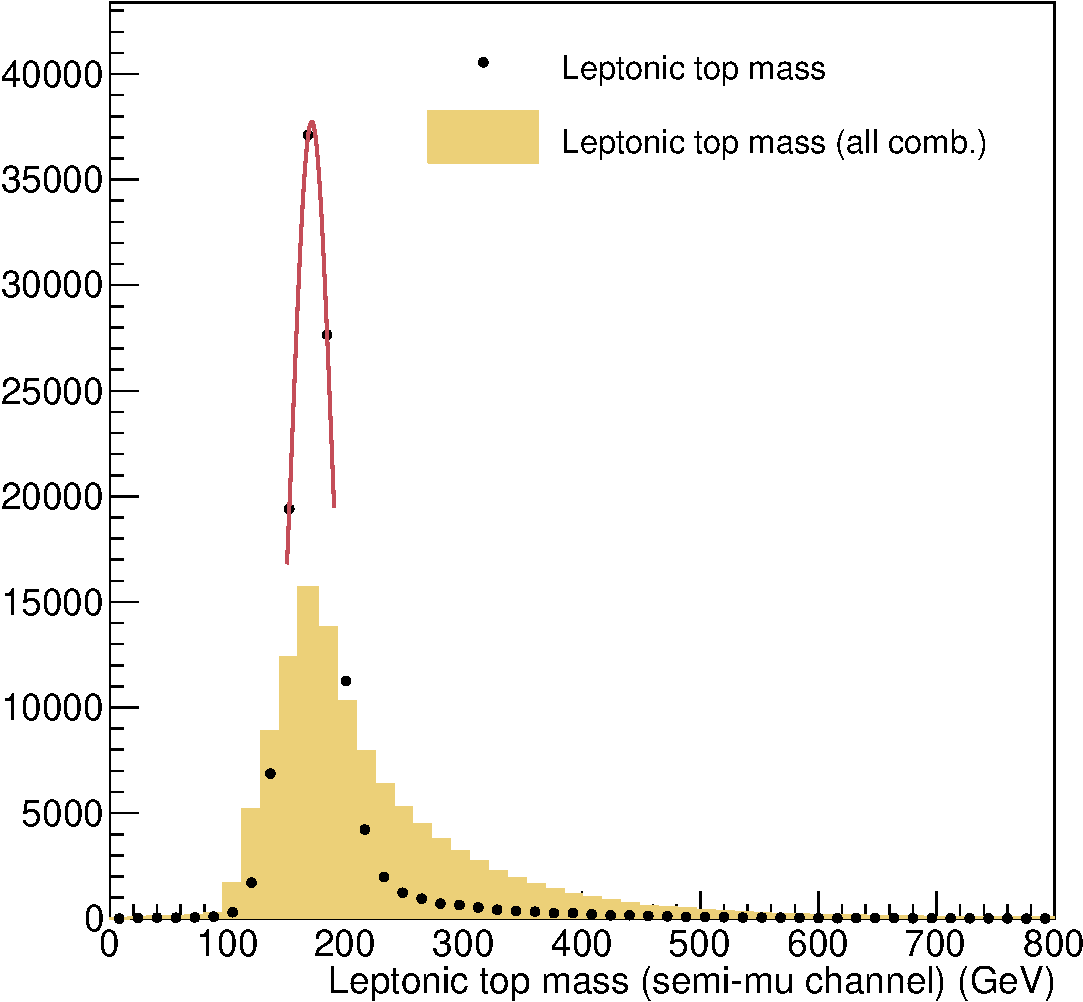
\includegraphics[width=0.41\textwidth]{chapitre6/figs/chi2/chi2_discrimant_combinations_leptonic_top_mass_mu.pdf}} \qquad
    \subcaptionbox{$m_{\Ptop}^{\text{lept.}}$ semi-e}[0.41\textwidth]{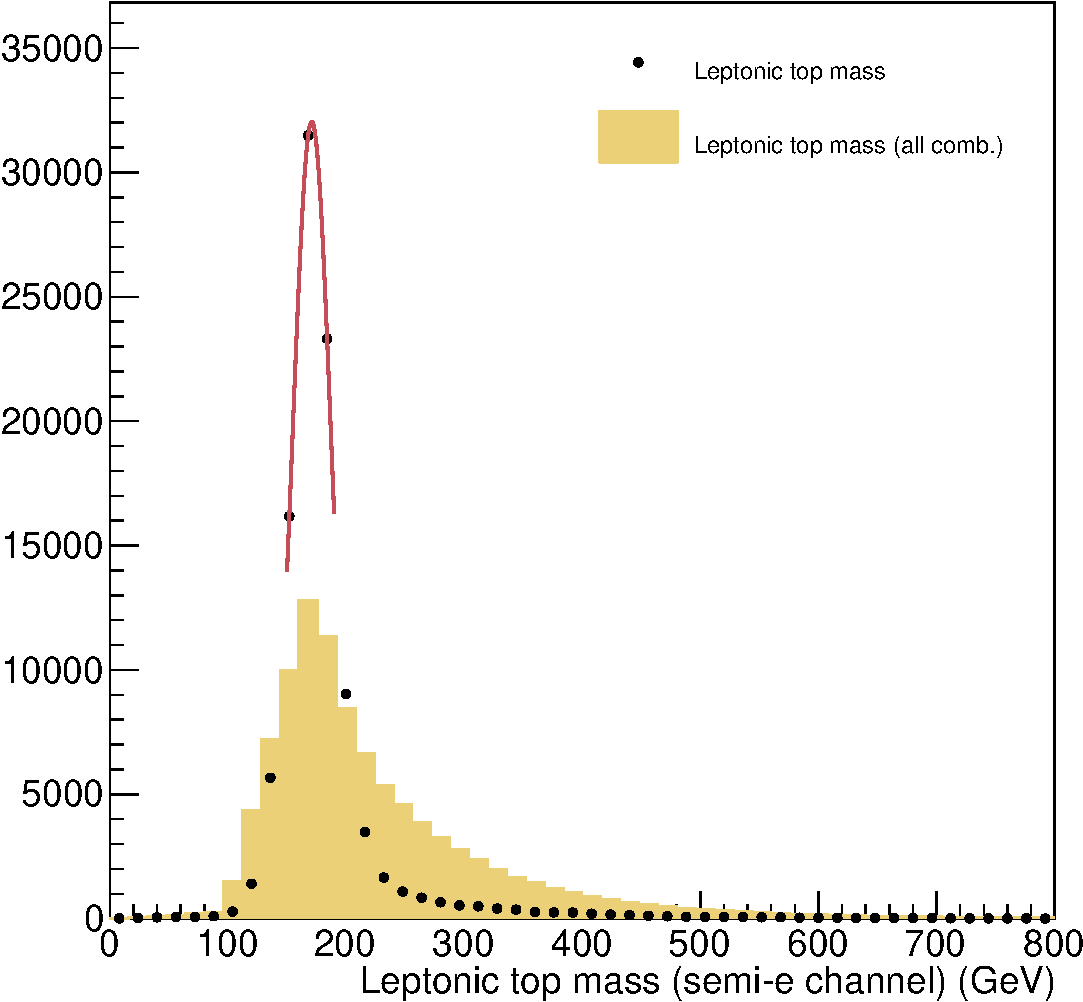
\includegraphics[width=0.41\textwidth]{chapitre6/figs/chi2/chi2_discrimant_combinations_leptonic_top_mass_e.pdf}} \\
    \subcaptionbox{$m_{\Ptop}^{\text{hadr.}}$}[0.41\textwidth]{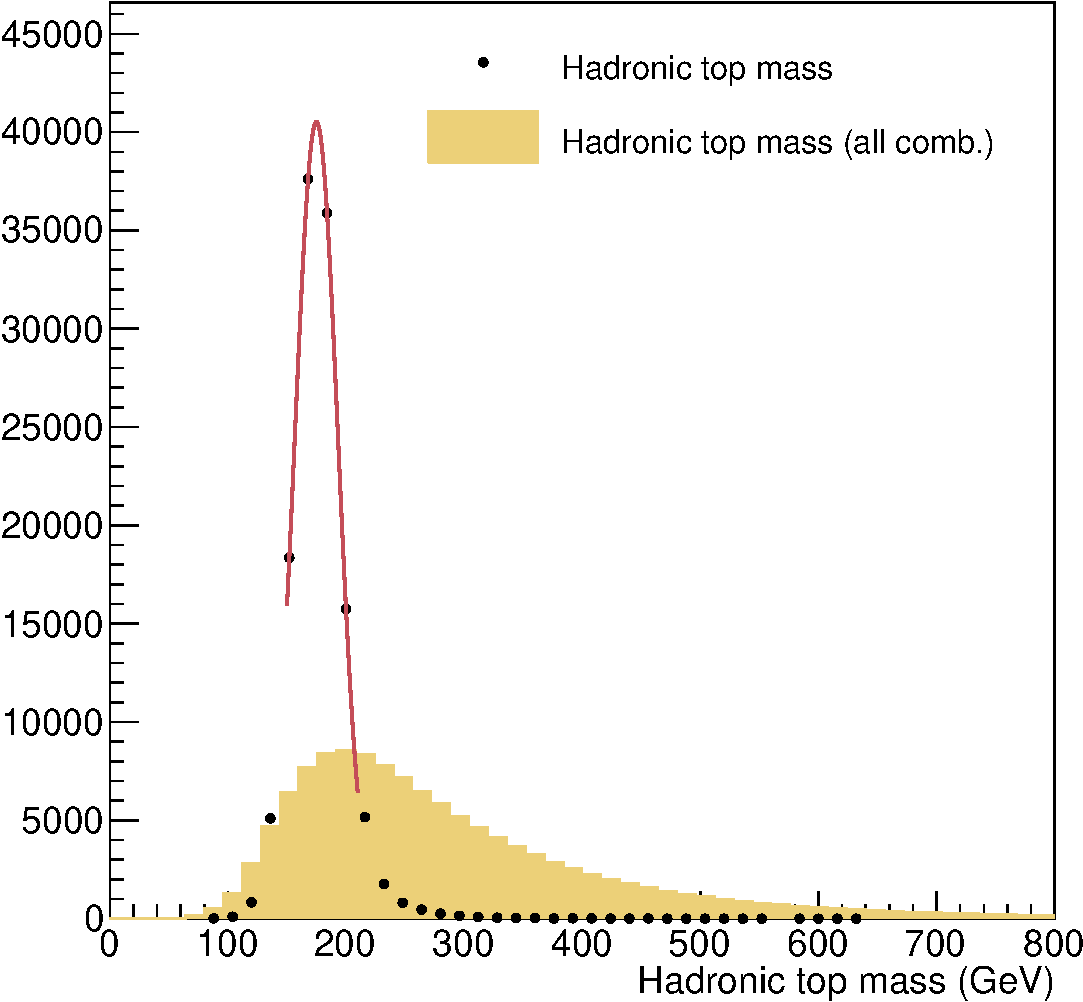
\includegraphics[width=0.41\textwidth]{chapitre6/figs/chi2/chi2_discrimant_combinations_hadronic_top_mass.pdf}} \qquad
    \subcaptionbox{$m_{\PW}^{\text{hadr.}}$}[0.41\textwidth]{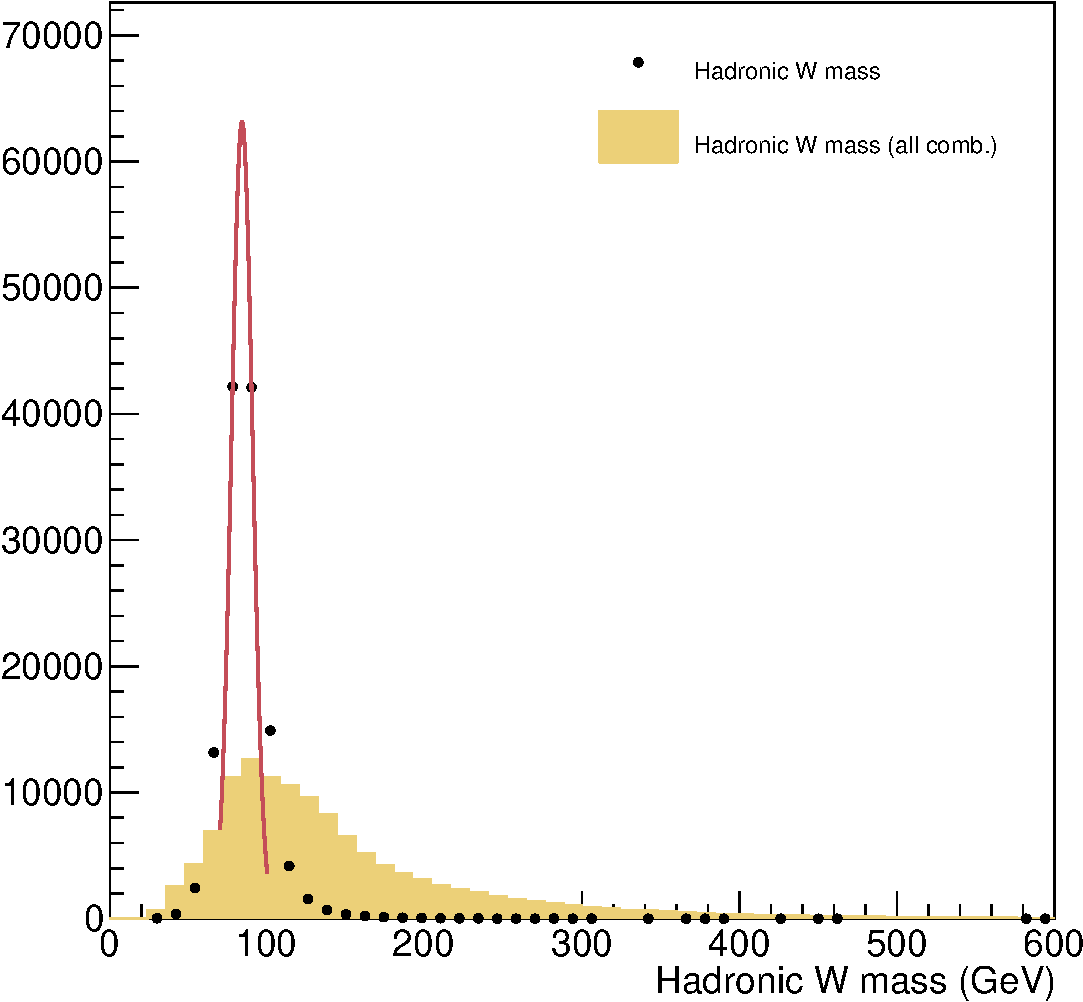
\includegraphics[width=0.41\textwidth]{chapitre6/figs/chi2/chi2_discrimant_combinations_w_mass.pdf}} \\
    \subcaptionbox{$H_{T}^{\text{frac.}}$}[0.41\textwidth]{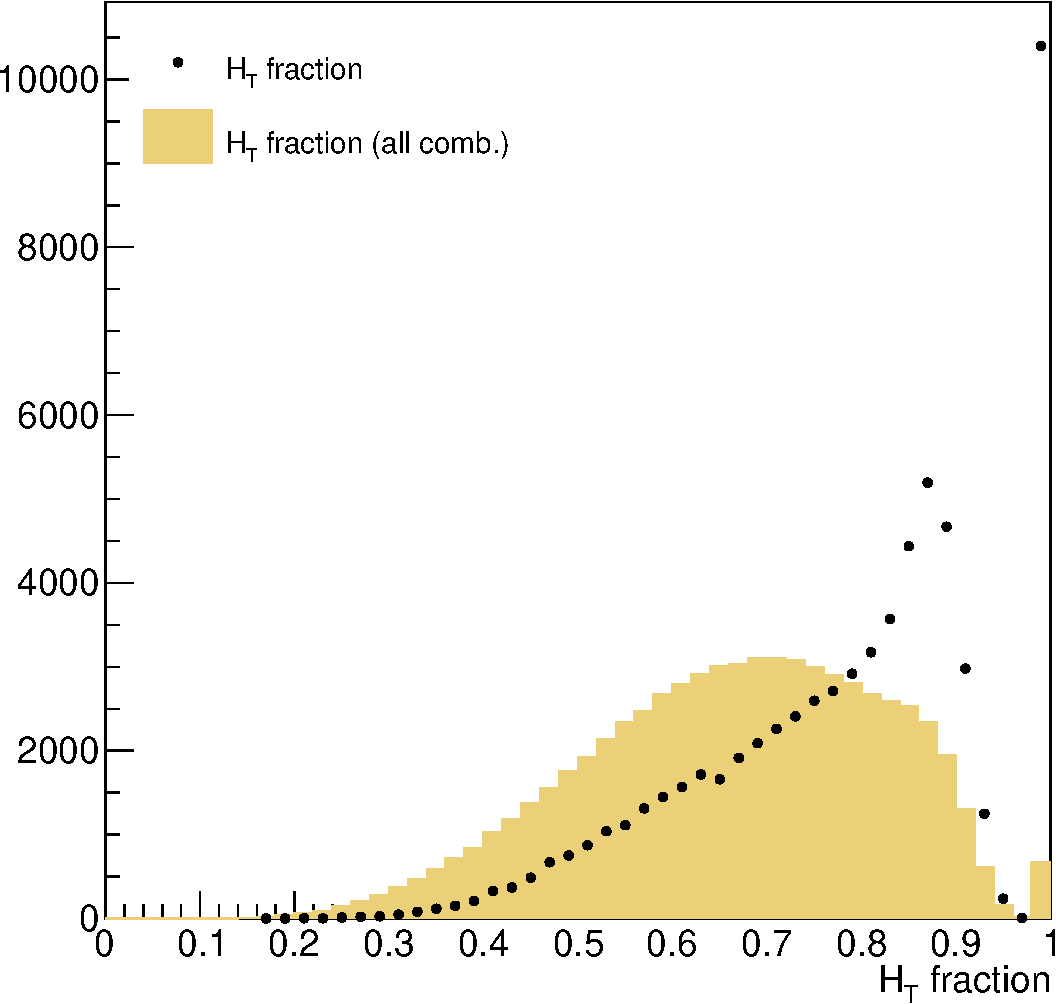
\includegraphics[width=0.41\textwidth]{chapitre6/figs/chi2/chi2_discrimant_combinations_ht_frac.pdf}}
    \caption{Distributions pour chaque discriminant du $\chi^2$. Les points noirs correspondent aux valeurs calculées en utilisant les bonne combinaisons de jets, à comparer avec les valeurs calculées en utilisant toutes les combinaisons de jets (histogramme jaune). Une interpolation gaussienne est superposée afin d'extraire les valeurs de références ainsi que leurs incertitudes.}
    \label{fig:chi2_distributions}
\end{figure}

Les valeurs de références des discriminants sont définies comme les valeurs les plus probables des discriminants sur la simulation. Afin d'extraire ces valeurs, on reconstruit l'événement \ttbar en utilisant uniquement la bonne association de jet. Cette bonne association est déterminée en utilisant la vérité Monte Carlo. À chaque jet reconstruit, on tente d'assigner un parton provenant de la désintégration \ttbar. Cette procédure d'assignation est réalisée en demandant que la distance entre le jet reconstruit et le parton dans le plan $(\eta, \phi)$ ($\Delta R = \sqrt{\Delta \eta^2 + \Delta \phi^2}$) soit inférieure à $0.4$, et que la différence d'impulsion transverse ($\Delta p_T$) soit inférieure à \SI{300}{\%}. Dans le cas où on ne peut pas associer les 4 quarks initiaux (\tilde \SI{60}{\%} des cas), l'événement n'est considéré ni pour les bonnes ni pour les mauvaises combinaisons.

\begin{table} \centering
    \begin{tabular}{@{}ccc@{}} \toprule
        Discriminant $x$& Valeur de référence $X_\text{MC}$ & Incertitude ($\sigma_\text{MC}$) \\ \midrule
        $m_{\Ptop}^{\text{lept.}}$ (semi-e) & \SI{170.88}{\GeV} & \SI{17.29}{\GeV} \\
        $m_{\Ptop}^{\text{lept.}}$ (semi-$\mu$) & \SI{170.94}{\GeV} & \SI{17.36}{\GeV} \\
        $m_{\Ptop}^{\text{hadr.}}$ & \SI{175.16}{\GeV} & \SI{17.35}{\GeV} \\
        $m_{\PW}^{\text{hadr.}}$ & \SI{84.06}{\GeV} & \SI{10.12}{\GeV} \\
        $H_{T}^{\text{frac.}}$ & \num{1} & \num{0.15} \\ \bottomrule
    \end{tabular}
    \caption{Valeurs de références et incertitudes pour chaque discriminant utilisé dans le calcul du $\chi^2$. Ces valeurs ont été déterminées sur des événements \ttbar simulés.}
    \label{tab:chi2_ref_values}
\end{table}

On évalue la valeur de chaque discriminant pour chaque bonne combinaison. La \cref{fig:chi2_distributions} présente les distributions de chaque discriminant. Les valeurs de référence et les incertitudes associées sont extraites grâce à une interpolation avec une fonction gaussienne (en rouge sur les figures). Seule la distribution de $H_T^\text{frac.}$ n'est pas gaussienne. Pour ce cas particulier, la valeur moyenne et la moyenne quadratique (RMS) de la distribution sont utilisées.

Le \cref{tab:chi2_ref_values} résume les valeurs de références utilisées pour le calcul du $\chi^2$, avec leurs incertitudes associées. Ces valeurs ont été déterminées sur des événements \ttbar simulés.

\bigskip

Le choix de la bonne combinaison de jets est effectuée de la façon suivante : pour chaque événement sélectionné, on itère sur tous les sous-ensembles de 4 jets de l'événement. Pour chaque sous-ensemble, on calcule pour toutes les combinaisons de jets la valeur du $\chi^2$. On retient au final la combinaison qui minimise le $\chi^2$. On peut voir \cref{fig:chi2_distribution} la distribution du $\chi^2$ pour toutes les combinaisons (gris) et pour la bonne combinaison (rouge). On voit que choisir la valeur du $\chi^2$ la plus petite permet de sélectionner majoritairement la bonne combinaison.

\begin{figure}[tbp] \centering
    \subcaptionbox{\label{fig:chi2_distribution}}[0.48\textwidth]{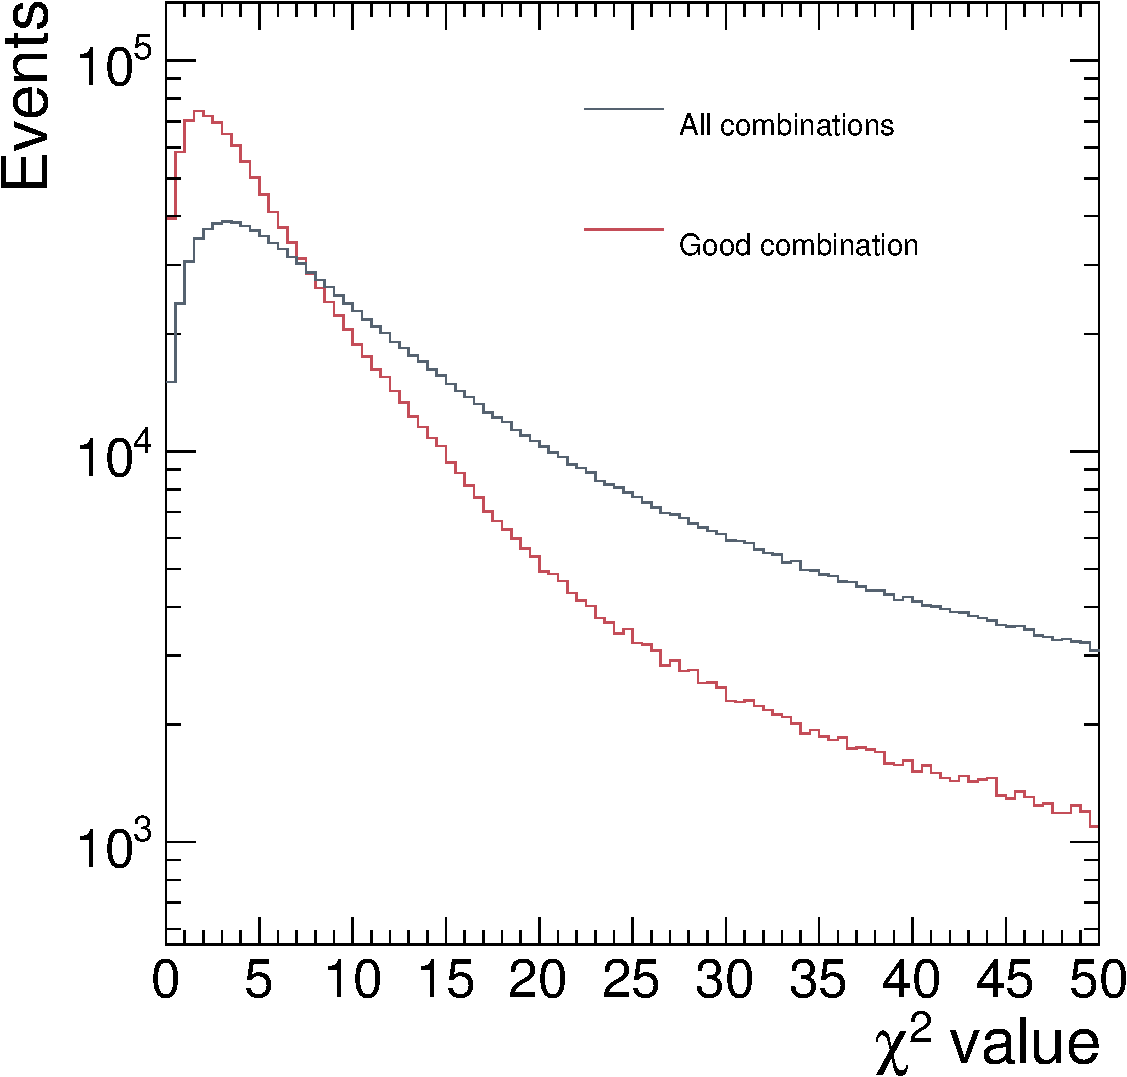
\includegraphics[width=0.48\textwidth]{chapitre6/figs/chi2/chi2_distribution.pdf}} \hfill
    \subcaptionbox{\label{fig:chi2_ptsyst}}[0.48\textwidth]{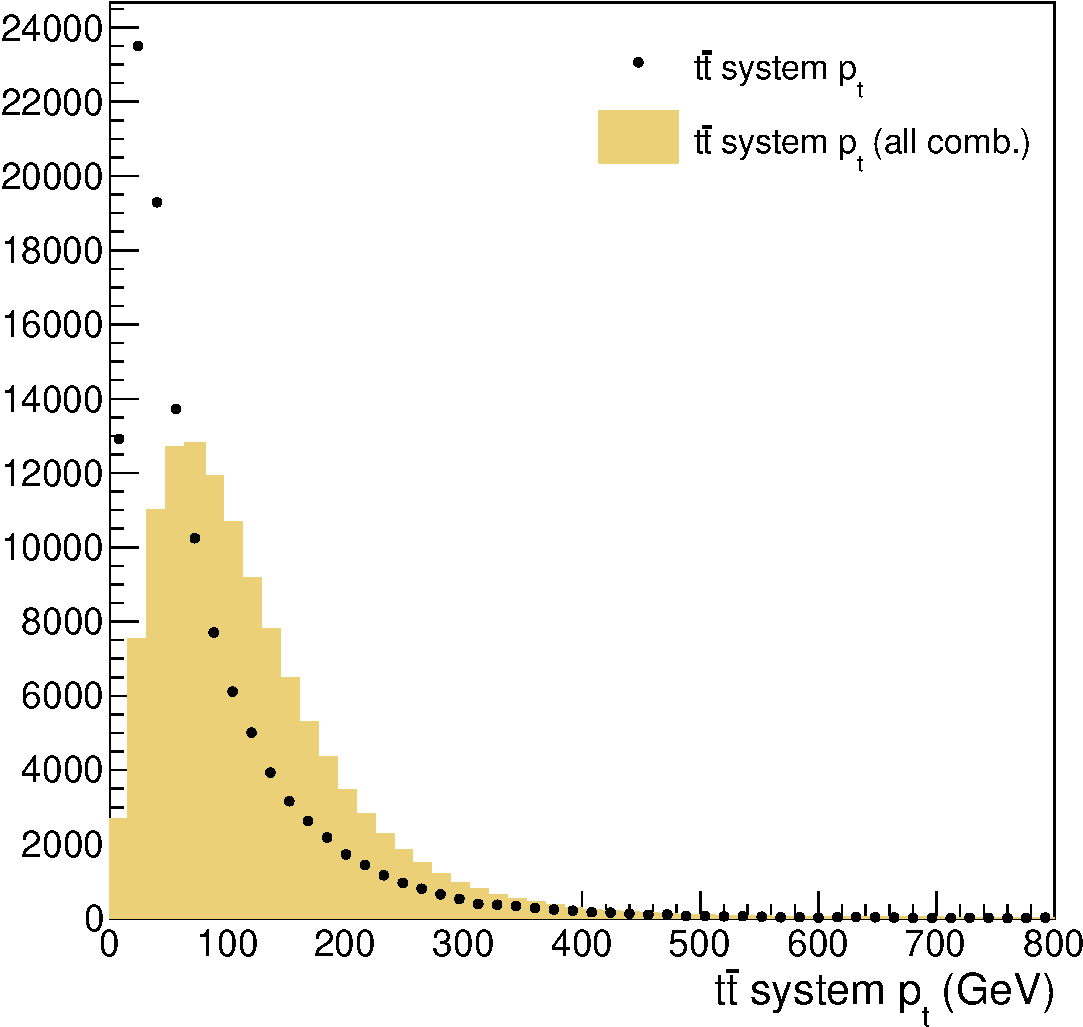
\includegraphics[width=0.48\textwidth]{chapitre6/figs/chi2/chi2_discrimant_combinations_pt_syst.pdf}}
    \caption{(\subref{fig:chi2_distribution}) Comparaison entre les distributions de $\chi^2$ pour toutes les combinaisons de jets (\textcolor{bleu_gris}{gris}) et pour la bonne combinaison de jets (\textcolor{rouge_grandmere}{rouge}), réalisée à partir d'événements \ttbar simulées. La courbe \textcolor{rouge_grandmere}{rouge} est normalisée au nombre d'événements de la courbe \textcolor{bleu_gris}{grise}. (\subref{fig:chi2_ptsyst}) $p_T$ du système \ttbar pour les bonnes combinaisons ainsi que toutes les combinaisons.}
\end{figure}

Pour pouvoir évaluer les performances de l'algorithme de tri par $\chi^2$, il est utile de donner quelques définitions :

\begin{itemize} \label{page:chi2_def}
    \item On parle d'\textbf{événement associable} s'il est possible d'associer à chaque parton de la désintégration \ttbar un jet reconstruit, selon la procédure détaillée ce-dessus.
    \item On parle d'\textbf{événement associé} si un événement est associable, et si l'algorithme de tri par $\chi^2$ a permis de choisir correctement les 4 jets provenant de la désintégration \ttbar. Pour cette classe d'événement, la position des jets n'est pas importante.
    \item Enfin, on parle d'\textbf{événement associé et bien placé} si un événement est associé, et si les 4 jets sélectionnés sont aussi bien placé, c'est-à-dire si le jet choisi pour être le jet \Pbottom leptonique est correct, etc.
\end{itemize}

\begin{figure}[tbp]
  \centering
  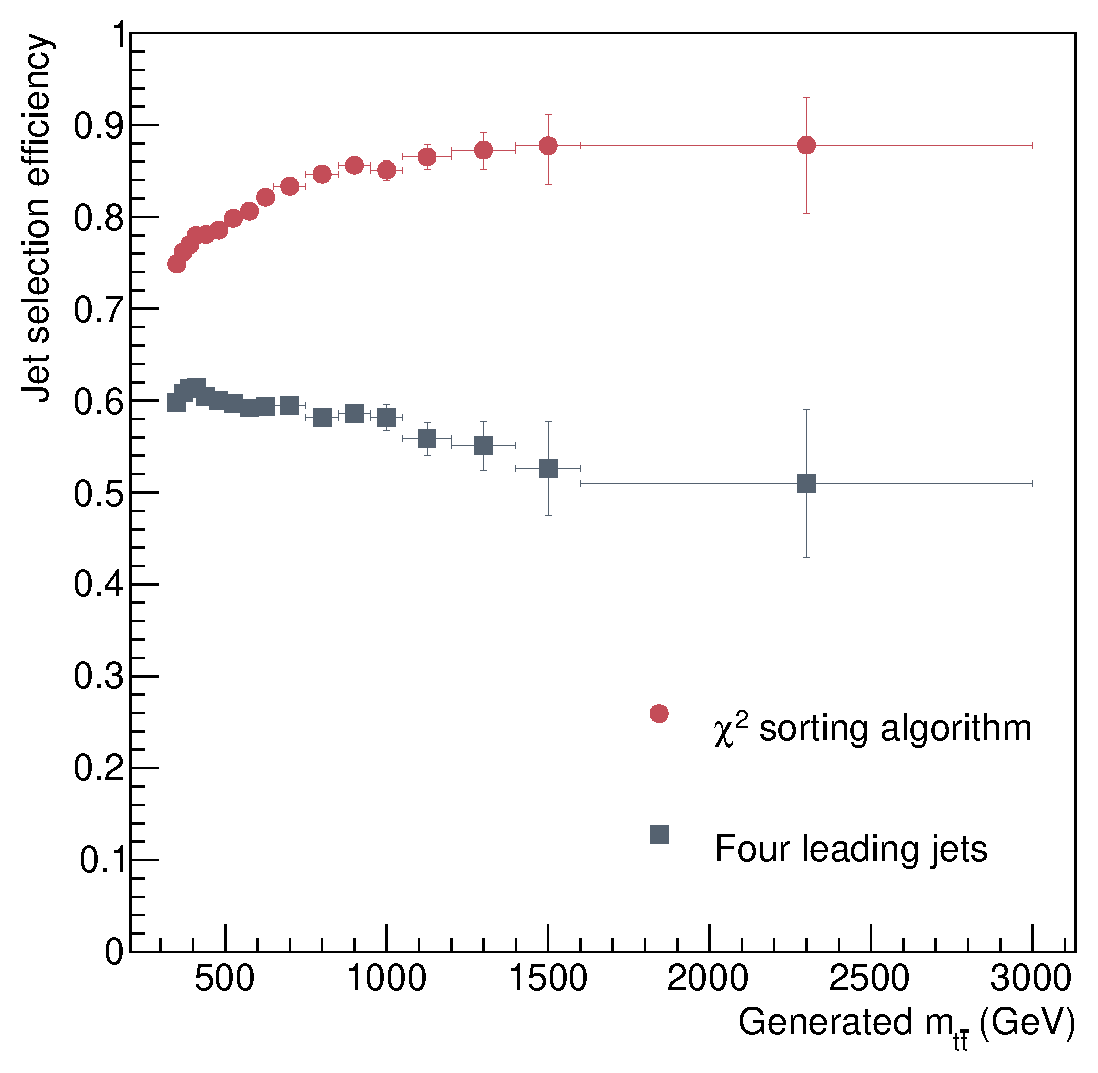
\includegraphics[width=0.48\textwidth]{chapitre6/figs/chi2/jet_selection_efficiency.pdf}
  \caption{ Évolution de l'efficacité d'obtenir un événement associé en fonction de la masse invariante \ttbar généré pour l'algorithme de tri par $\chi^2$ (\textcolor{rouge_grandmere}{rouge}) ou en sélectionnant simplement les 4 jets de plus haute impulsions (\textcolor{bleu_gris}{gris}).}
  \label{fig:chi2_vs_jets}
\end{figure}

Lorsque l'on reconstruit la masse invariante \ttbar, on reconstruit la masse invariante d'un système à 6 corps (voir \cref{eq:invariant_mass_tt}). La position des jets sélectionnés n'a au final aucune influence sur la valeur de la masse invariante. Seul importe le fait de choisir les 4 bons jets. On cherche donc à maximiser l'efficacité d'obtenir la bonne combinaison de jets. Pour cela, on cherche à savoir si l'ajout d'un autre terme dans le $\chi^2$ permet d'améliorer cette efficacité. L'étude s'est concentrée sur la possible d'ajouter le $p_T$ du système \ttbar comme variable discriminante. On peut voir \cref{fig:chi2_ptsyst} le pouvoir de discrimination d'une telle variable. Les résultats de cette étude sont présentés \cref{tab:chi2_study}. En ajoutant une variable supplémentaire, l'efficacité diminue de près d'\SI{1}{\%}. Le choix a donc été fait de garder le $\chi^2$ tel que présenté \cref{eq:chi2}.

\begin{table}[h] \centering
    \begin{tabular}{@{}ccccc@{}} \toprule
        & sans $H_{T}^{\text{frac.}}$ ni $p_{T}^{\ttbar}$ & avec $p_{T}^{\ttbar}$ & avec $H_{T}^{\text{frac.}}$ & avec $H_{T}^{\text{frac.}}$ et $p_{T}^{\ttbar}$ \\ \midrule
        $\epsilon_\text{associable}$ & \multicolumn{4}{c}{\SI{39.90 \pm 0.09}{\%}} \\
        $\epsilon_\text{associé}$ & \SI{75.92 \pm 0.13}{\%} & \SI{76.30 \pm 0.12}{\%} & \SI{79.55 \pm 0.12}{\%} & \SI{78.99 \pm 0.12}{\%} \\
        $\epsilon_\text{associé et bien placé}$ & \SI{41.63 \pm 0.15}{\%} & \SI{41.96 \pm 0.14}{\%} & \SI{44.04 \pm 0.14}{\%} & \SI{43.75 \pm 0.14}{\%} \\ \bottomrule
    \end{tabular}
    \caption{Efficacité d'obtenir un événement associable ($\epsilon_\text{associable}$), un événement associé ($\epsilon_\text{associé}$) et un événement associé et bien placé ($\epsilon_\text{associé et bien placé}$) pour différentes configurations du $\chi^2$. La configuration optimale est celle utilisant uniquement le terme supplémentaire $H_{T}^{\text{frac.}}$.}
    \label{tab:chi2_study}
\end{table}

D'autres méthodes existent pour sélectionner la bonne combinaison de jets. La plus simple d'entre elle consiste à sélectionner les 4 jets de plus haute impulsion. On compare \cref{fig:chi2_vs_jets} les performances de l'algorithme de tri par $\chi^2$ par rapport cette méthode. On constate que l'algorithme de tri par $\chi^2$ est bien plus performant que le simple choix des 4 jets, avec une différence d'efficacité variant entre \tilde\SI{15}{\%} et \tilde\SI{30}{\%} en fonction de la masse invariante \ttbar générée.

% \begin{figure}[tbp] \centering
%     \subcaptionbox{\label{fig:chi2_vs_jets}}[0.48\textwidth]{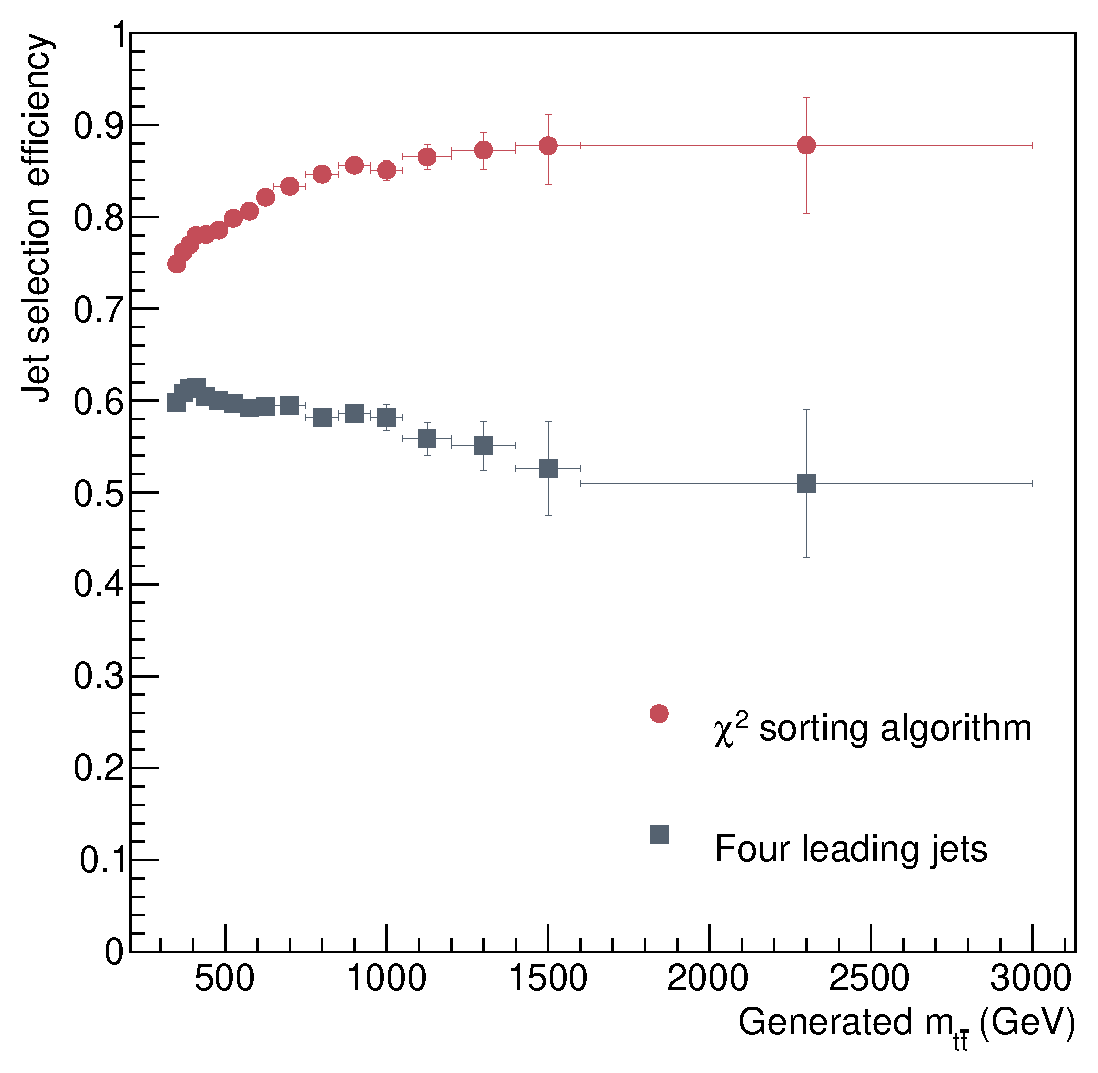
\includegraphics[width=0.48\textwidth]{chapitre6/figs/chi2/jet_selection_efficiency.pdf}}
%     \caption{(\subref{fig:chi2_vs_jets}) Évolution de l'efficacité d'obtenir un événement associé en fonction de la masse invariante \ttbar généré pour l'algorithme de tri par $\chi^2$ (\textcolor{rouge_grandmere}{rouge}) ou en sélectionnant simplement les 4 jets de plus haute impulsions (\textcolor{bleu_gris}{gris}).}
%     \label{fig:label}
% \end{figure}

\subsection{Algorithme de tri par MVA}

Des nombreuses variables rentrent en jeu lors du calcul de la masse invariante \ttbar. Une méthode simple pour les exploiter serait d'étendre le $\chi^2$ (\cref{eq:chi2}) pour ajouter autant de termes que nécessaire. Cela suppose néanmoins que les variables que l'on utilise comme discriminant soient gaussiennes, ce qui est le cas pour des distributions de masses invariantes, mais pas pour d'autres variables, telles que $\Delta \phi$ entre deux objets, ou l'impulsion transverse d'un autre objet.

Afin d'exploiter toutes les informations possibles pour discriminer entre bonnes et mauvaises combinaisons, une analyse multi-variée a été mise en place, utilisant comme algorithmes les arbres de décisions boostés (BDT, \emph{Boosted Decision Tree}) et un réseau de neurones (NN, \emph{Neural Network}).

%Deux algorithmes différents sont comparées dans cette section : les arbres de décisions boostés (BDT, \emph{Boosted Decision Tree}) et les réseaux de neurones (NN, \emph{Neural Network}).

\subsubsection{Arbres de décisions boostés}

Un arbre de décision est un algorithme de classification des événements utilisant en entrée plusieurs variables, et qui permet en sortie de classer les événements en deux catégories distinct : "signal" ou "fond". L'algorithme commence au nœud racine, où une première coupure sur une variable $x_i$ est appliquée.Une deuxième coupure sur une variable $x_j$ est ensuite appliquée, qui dépend du résultat de la première coupure: on obtient ainsi 2 nouveaux noeuds. Cette procédure est répétée jusqu'à ce qu'une condition d'arrêt soit atteinte. L'événement est alors classé "signal" ou "fond". Un exemple d'arbre de décision est présenté \cref{fig:bdt}.

Afin de construire un tel arbre, une phase d'entrainement est nécessaire. Cette entrainement est réalisé à la fois sur des événements classés comme "signal" et sur des événements classés comme "fond". Un des principaux problèmes de cet algorithme est son instabilité vis-à-vis des fluctuations statistiques dans l'échantillon utilisé pour l'entrainement. Par exemple, si deux variables font preuves d'un pouvoir de discrimination similaire, une fluctuation statistique pourrait décider l'algorithme à utiliser la première variable au lieu de la deuxième.

Le problème est contourné en construisant une "forêt" d'arbres de décision. La classification d'un événement en "signal" ou "fond" est déterminée par le résultat majoritaire sur tous les arbres. L'entrainement de chaque arbre est réalisé sur le même échantillon. La seule différence vient de l'application d'un poids particulier à chaque événement : les événements mal classés durant l'entrainement de l'arbre de décision auront un poids plus grand lors de l'entrainement de l'arbre suivant. Cette technique est appelé \emph{boost} \citep{Freund1997119} et permet de stabiliser l'algorithme.

\begin{figure}[t!] \centering
    \subcaptionbox{Vue schématique d'un arbre de décision. En commençant au nœud racine, une suite de sélections binaires sont appliquées en utilisant le discriminant $x_i$, qui peut varier ou non à chaque nœud de la sélection. A la fin de chaque branche de sélection, l'événement est classé comme "signal" (S) ou comme "fond" (B). \label{fig:bdt}}[0.48\textwidth]{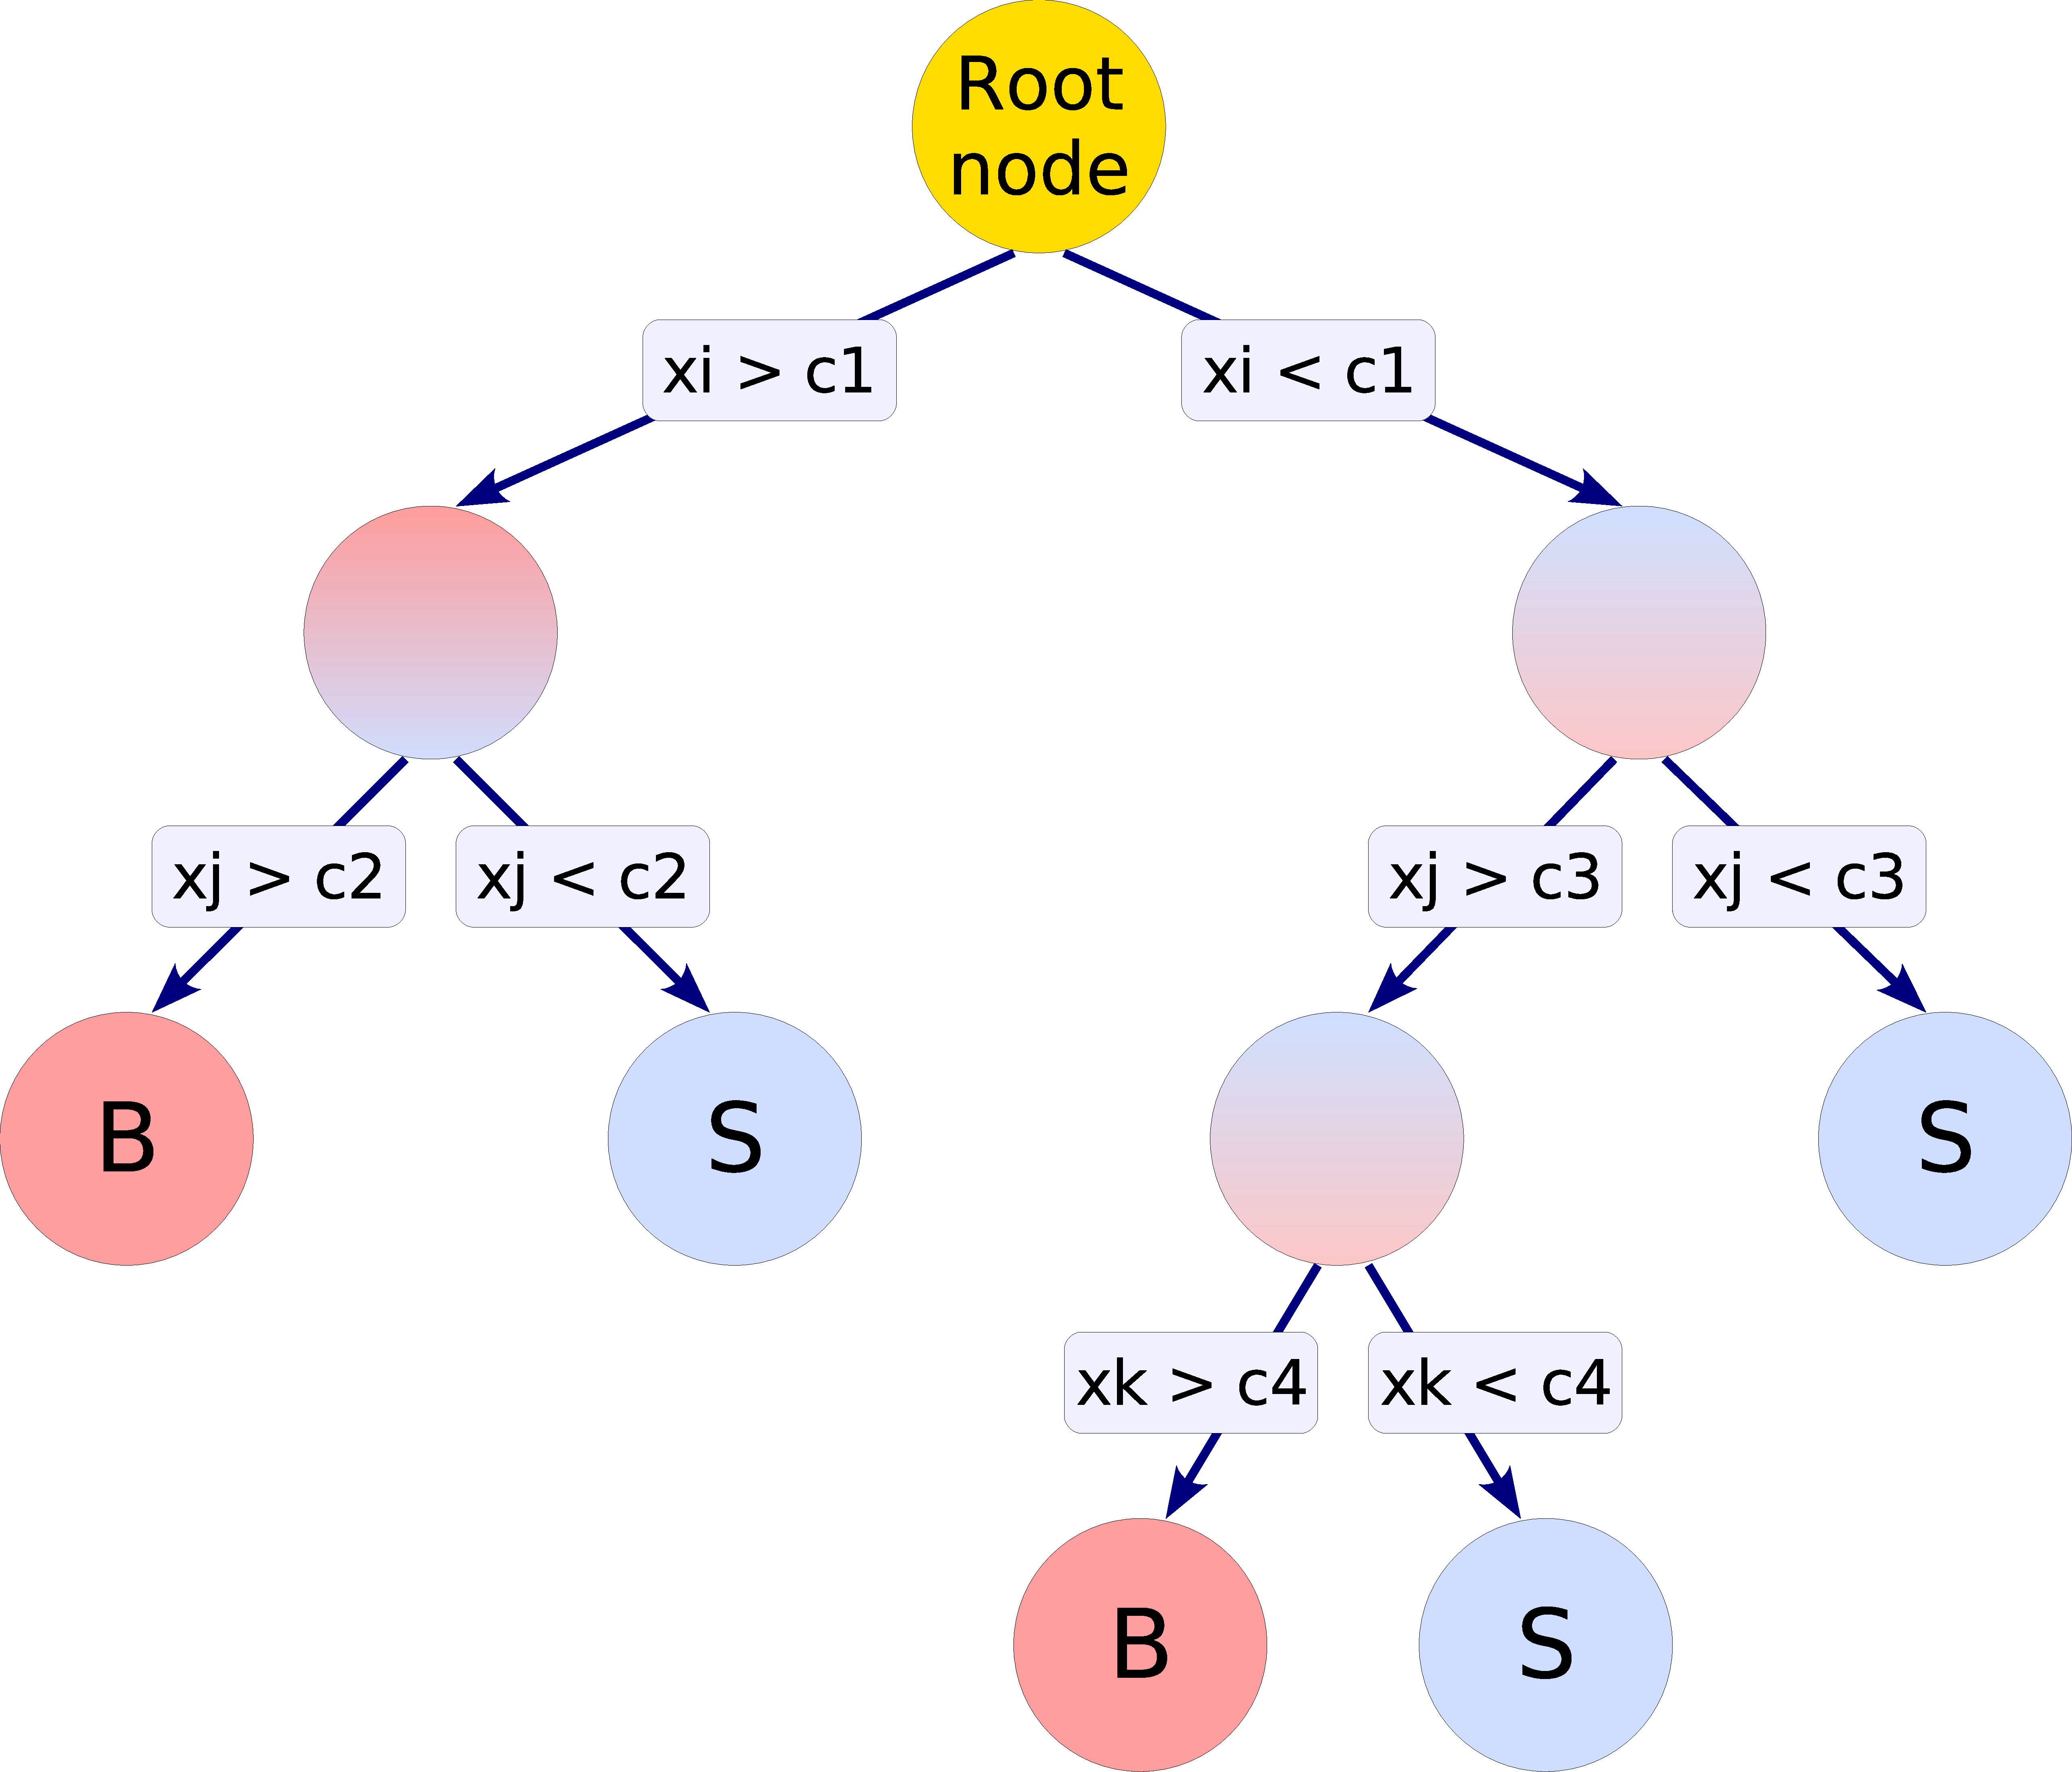
\includegraphics[width=0.48\textwidth]{chapitre6/figs/BDT.pdf}} \hfill
    \subcaptionbox{Vue schématique d'un réseau de neurones. En vert, deux neurones d'entrées sont connectés à des neurones "cachés" (bleu), eux même connectés à un neurone de sortie (jaune). \label{fig:nn}}[0.48\textwidth]{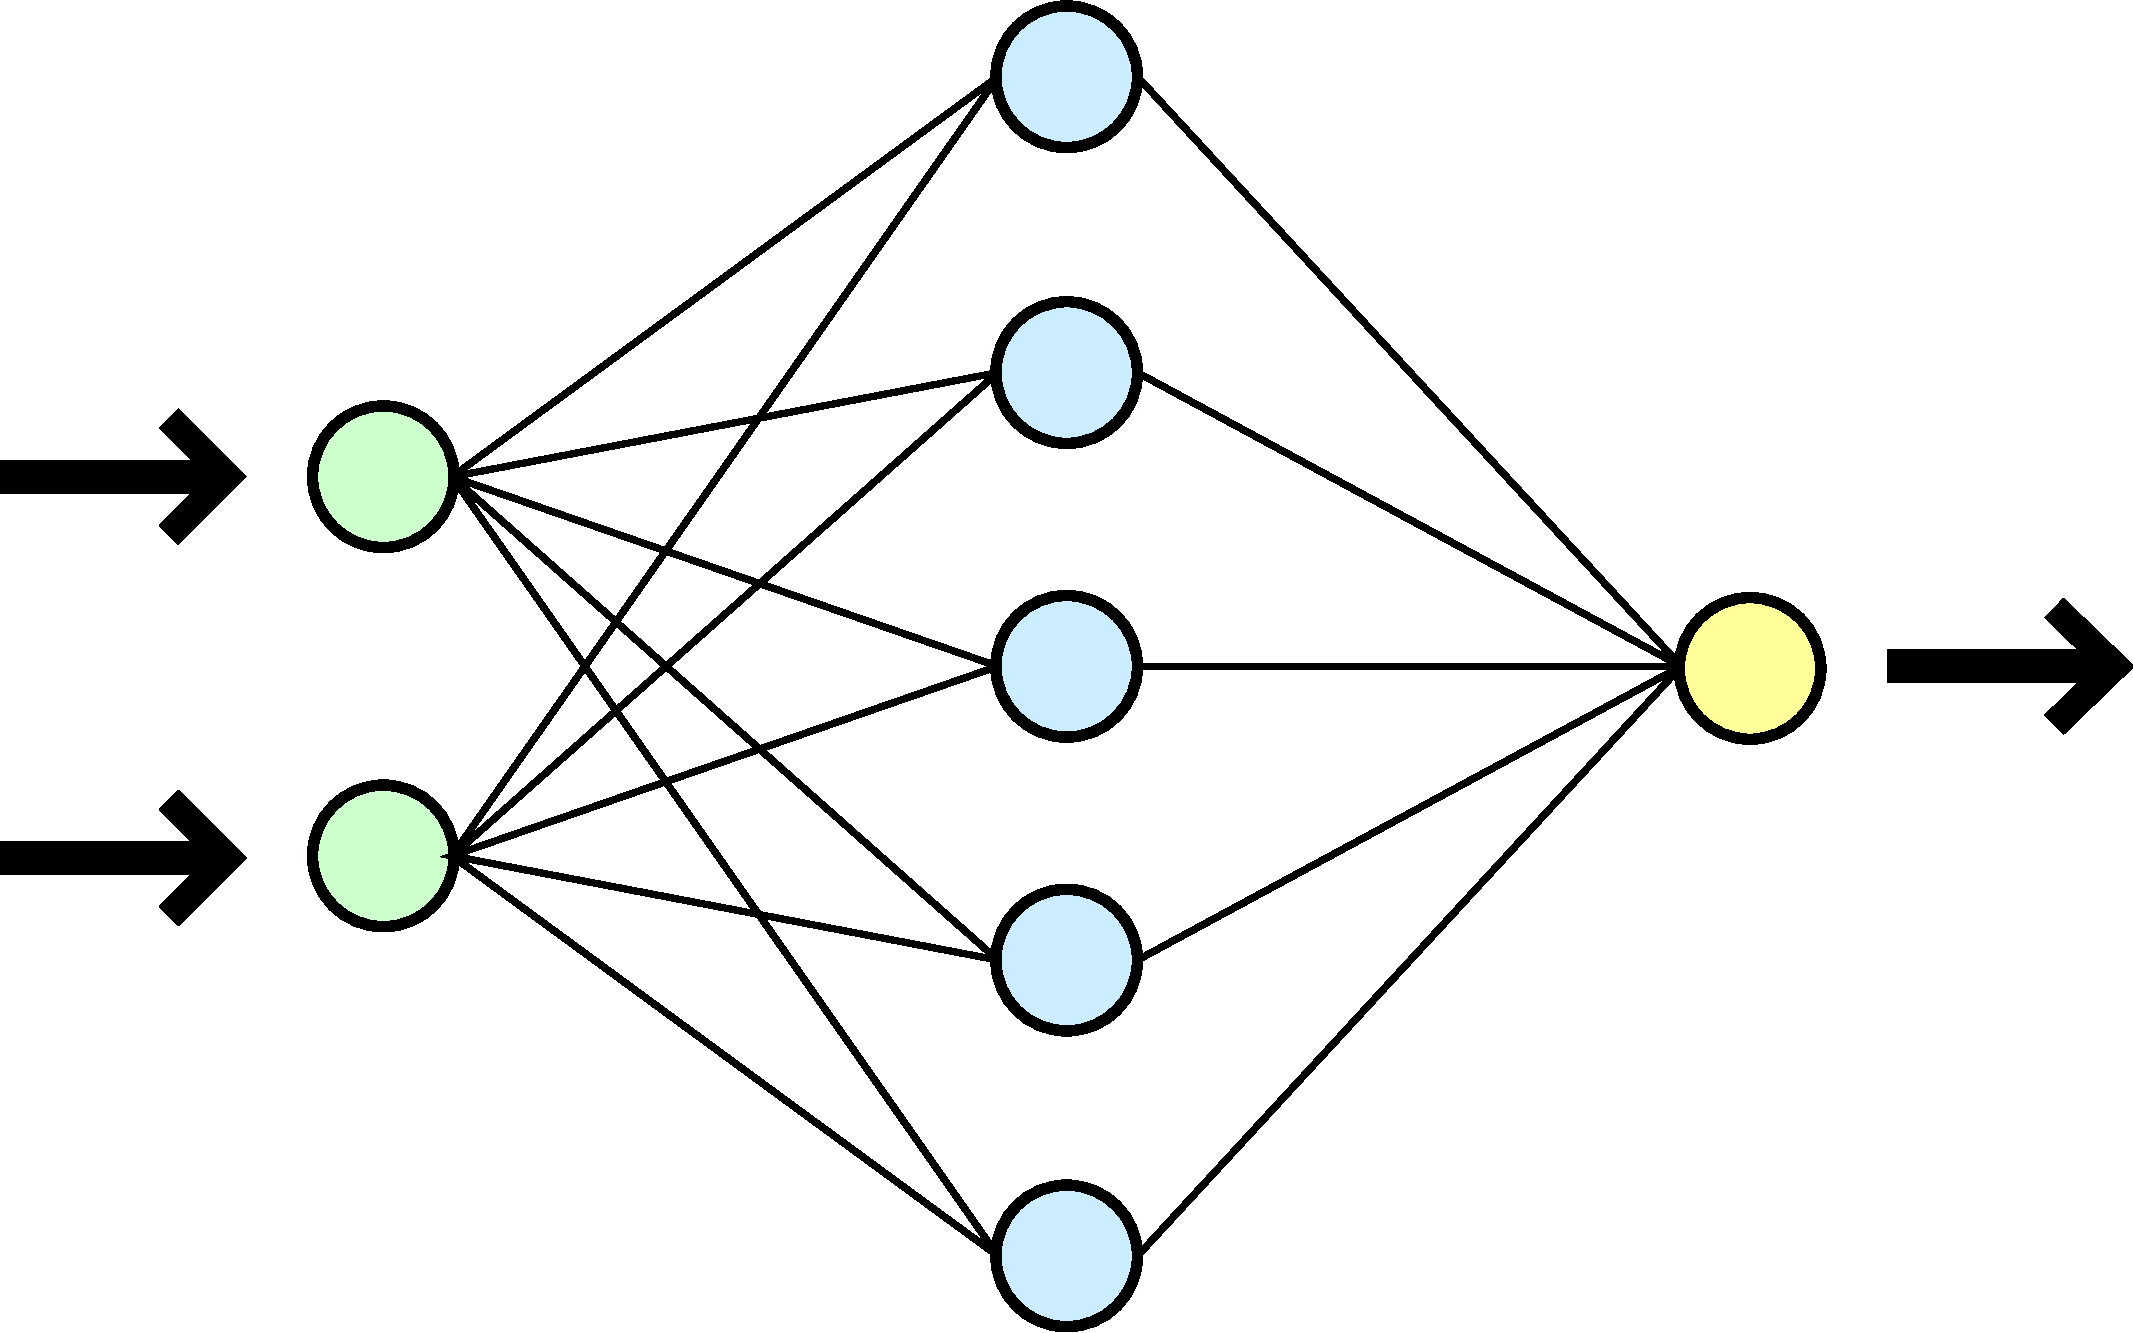
\includegraphics[width=0.48\textwidth]{chapitre6/figs/Neural_network.pdf}}
    \caption{Vue schématique de deux algorithmes de MVA.}
\end{figure}

\subsubsection{Réseau de neurones}

Un réseau de neurones consiste en une collection interconnectée de neurones, où chaque neurone dispose d'une fonction de transfert transformant une valeur d'entrée en valeur de sortie. En utilisant plusieurs couches de neurones, il est possible de créer un réseau complexe qui permet de classer des événements. La \cref{fig:nn} présente une vue schématique d'un réseau de neurones.

\subsubsection{Classification des événements \ttbar}

L'utilisation d'un MVA permet de classer un événement en deux catégories : "signal" ou "fond". Pour notre cas particulier, la catégorie "signal" correspond au choix de la bonne combinaison de jets, et "fond" aux mauvaises combinaisons. Les variables rentrant dans la composition du MVA sont exactement les mêmes que celles de l'algorithme de $\chi^2$. Utiliser des variables angulaires ou cinématiques est possible, mais rend l'algorithme MVA dépendant du mode de production des paires \ttbar. Or, on souhaite pouvoir utiliser cet algorithme sur des processus de nouvelle physique : on doit donc garder l'algorithme le plus indépendant possible du mode de production.

\bigskip

\begin{figure}[tbp] \centering
    \subcaptionbox{\label{fig:mva_bdt_discr}}[0.48\textwidth]{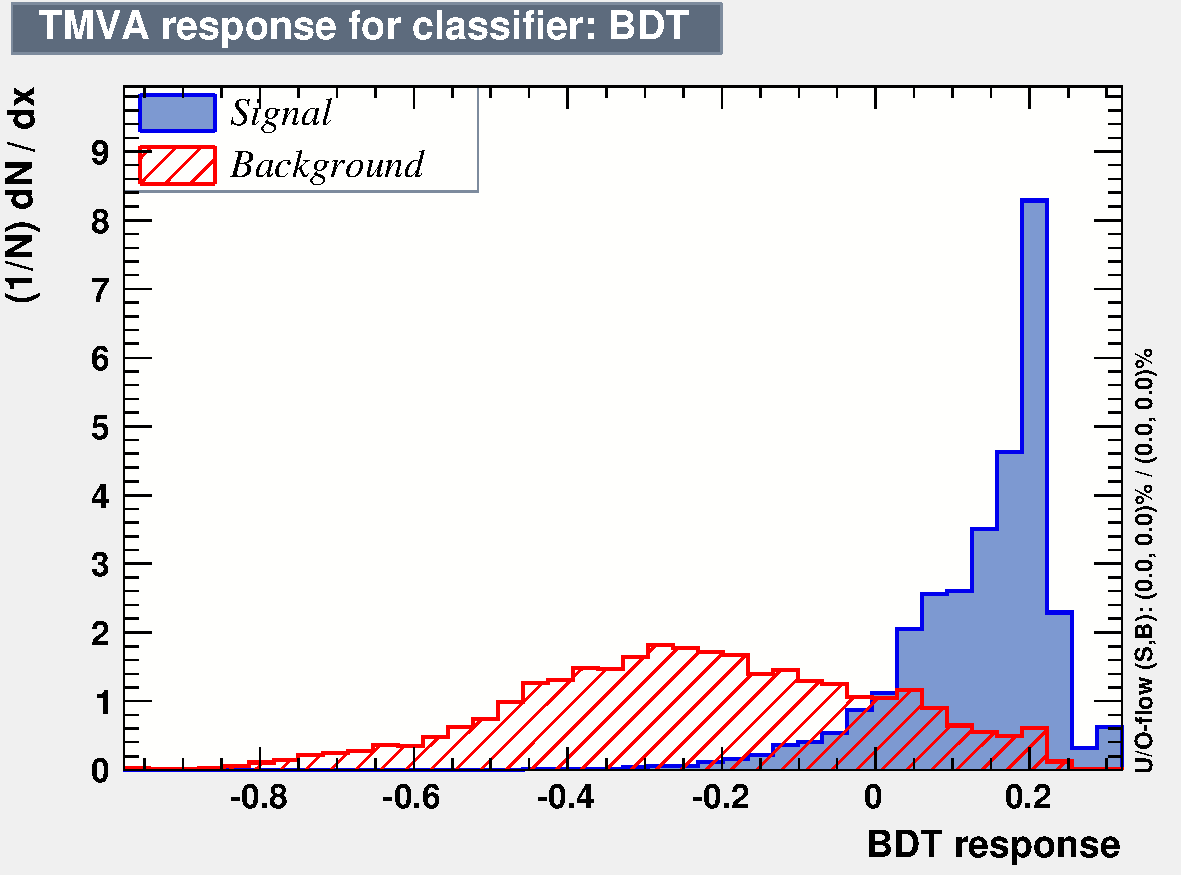
\includegraphics[width=0.48\textwidth]{chapitre6/figs/mva/mva_BDT.pdf}}
    \subcaptionbox{\label{fig:mva_nn_discr}}[0.48\textwidth]{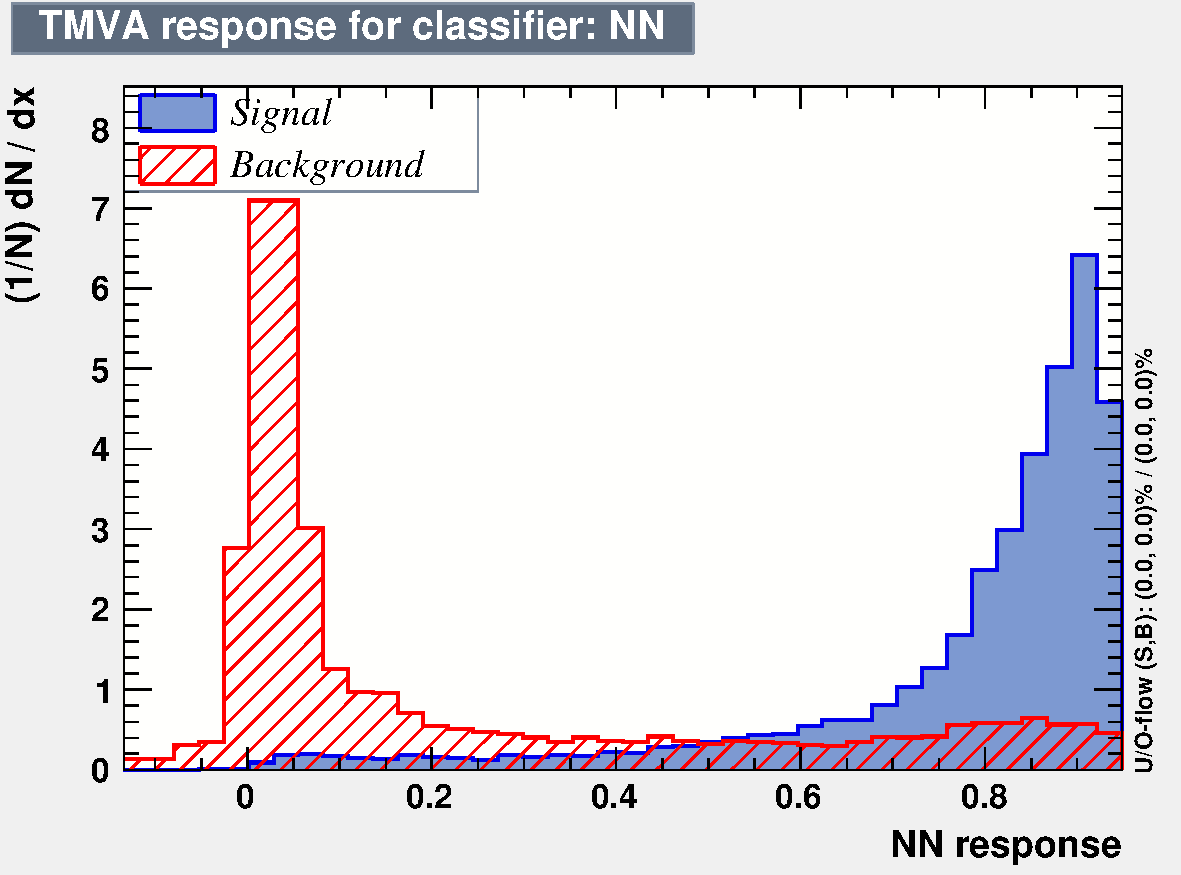
\includegraphics[width=0.48\textwidth]{chapitre6/figs/mva/mva_NN.pdf}}
    \caption{Valeurs de sortie pour les bonnes (bleu) et mauvaises (rouge) combinaisons, pour l'algorithme BDT (\subref{fig:mva_bdt_discr}) et le réseau de neurones (\subref{fig:mva_nn_discr}).}
\end{figure}

Les \cref{fig:mva_bdt_discr,fig:mva_nn_discr} présentent les valeurs de sorties de chaque MVA. On constate l'excellente discrimination entre les bonnes et mauvaises combinaisons. On identifie ici la bonne combinaison celle qui possède la plus grande valeur de sortie du MVA. Le \cref{tab:chi2_vs_bdt_vs_nn} résume les efficacités de sélectionner la bonne combinaison de jets pour l'algorithme de tri par $\chi^2$, pour le BDT et le NN. Malgré un très bon pouvoir de discrimination, l'algorithme de tri par $\chi^2$ reste plus performant que les deux MVA.

\begin{table}[tbp] \centering
    \sisetup{separate-uncertainty = true}
    \begin{tabular}{@{}cccc@{}} \toprule
        & $\chi^2$ & BDT & NN \\ \midrule
        $\epsilon_\text{associé}$ & \SI{80.23 \pm 1.08}{\%} & \SI{78.12 \pm 1.17}{\%} & \SI{74.33 \pm 1.18}{\%} \\
        $\epsilon_\text{associé et bien placé}$ & \SI{44.27 \pm 1.34}{\%} & \SI{44.56 \pm 1.34}{\%} & \SI{38.51 \pm 1.31}{\%} \\ \bottomrule
    \end{tabular}
    \caption{Efficacité d'obtenir un événement associé ($\epsilon_\text{associé}$) et un événement associé et bien placé ($\epsilon_\text{associé et bien placé}$) pour différentes configurations du $\chi^2$. La configuration optimale est celle utilisant uniquement le terme supplémentaire $H_{T}^{\text{frac.}}$.}
    \label{tab:chi2_vs_bdt_vs_nn}
\end{table}



\bigskip

L'étude dédiée au MVA est encore très préliminaire. De nombreuses améliorations sont possibles, comme par exemple optimiser la liste des variables en entrée afin d'améliorer encore la discrimination entre bonnes et mauvaises combinaisons. Avant que ces études ne soient menées, il a été décidé de ne pas utiliser de MVA en raison des moins bonnes performances par rapport à l'algorithme de tri par $\chi^2$.

\section{Performances de la reconstruction de la masse invariante} \label{sec:perf_reco_tt}

Deux critères sont utilisés afin de déterminer la qualité de la reconstruction de la masse invariante. Le plus important est la résolution, définie comme la différence entre la masse invariante reconstruite ($\mtt^\text{reco}$) et la masse invariante générée ($\mtt^\text{gen}$). Ainsi, plus la reconstruction est de qualité, plus la résolution est faible. On peut aussi observer la linéarité de la reconstruction, en traçant l'évolution de $\mtt^\text{reco}$ en fonction de $\mtt^{gen}$. Cette section est dédiée à la comparaison de ces deux critères pour l'algorithme de tri par $\chi^2$ ainsi que pour le BDT. À cause des faibles performances du réseau de neurones, cet algorithme n'est pas inclut dans cette étude.

\bigskip

La \cref{fig:mtt_reso_chi2} présente la résolution obtenue avec l'utilisation de l'algorithme de tri par $\chi^2$ sur la masse invariante \mtt. Il est intéressant de comparer ce résultat avec l'utilisation des quatre jets de plus grande impulsion de l'événement pour reconstruire la masse invariante. Les performances de ces deux algorithmes sont présentées dans la \cref{fig:mtt_reso_chi2_vs_four_jets}. La \cref{fig:mtt_response_chi2_vs_four_jets} montre la linéarité de la reconstruction pour ces deux algorithmes, tandis que la \cref{fig:mtt_reso_vs_mtt_gen_chi2_vs_four_jets} présente l'évolution de la résolution en fonction de $\mtt^\text{gen}$. On peut observer deux effets opposés : utiliser l'algorithme de tri par $\chi^2$ permet d'améliorer la résolution d'environ \SI{2}{\%}, au détriment d'une légère perte de linéarité. Le critère de résolution est cependant plus important que la linéarité, puisqu'on cherche à détecter des résonances dans le spectre de masse invariante : une résonance plus étroite est plus aisée à détecter qu'une résonance large. À l'augmentation de la résolution s'ajoute aussi un élargissement des queues de la distribution de résolution, comme on peut le voir en comparant la \cref{fig:mtt_reso_four_jets} à la \cref{fig:mtt_reso_chi2}. L'utilisation de l'algorithme par $\chi^2$ permet donc d'améliorer significativement le spectre de masse invariante reconstruit.

\begin{figure}[tbp] \centering
    \subcaptionbox{\label{fig:mtt_reso_chi2}}[0.48\textwidth]{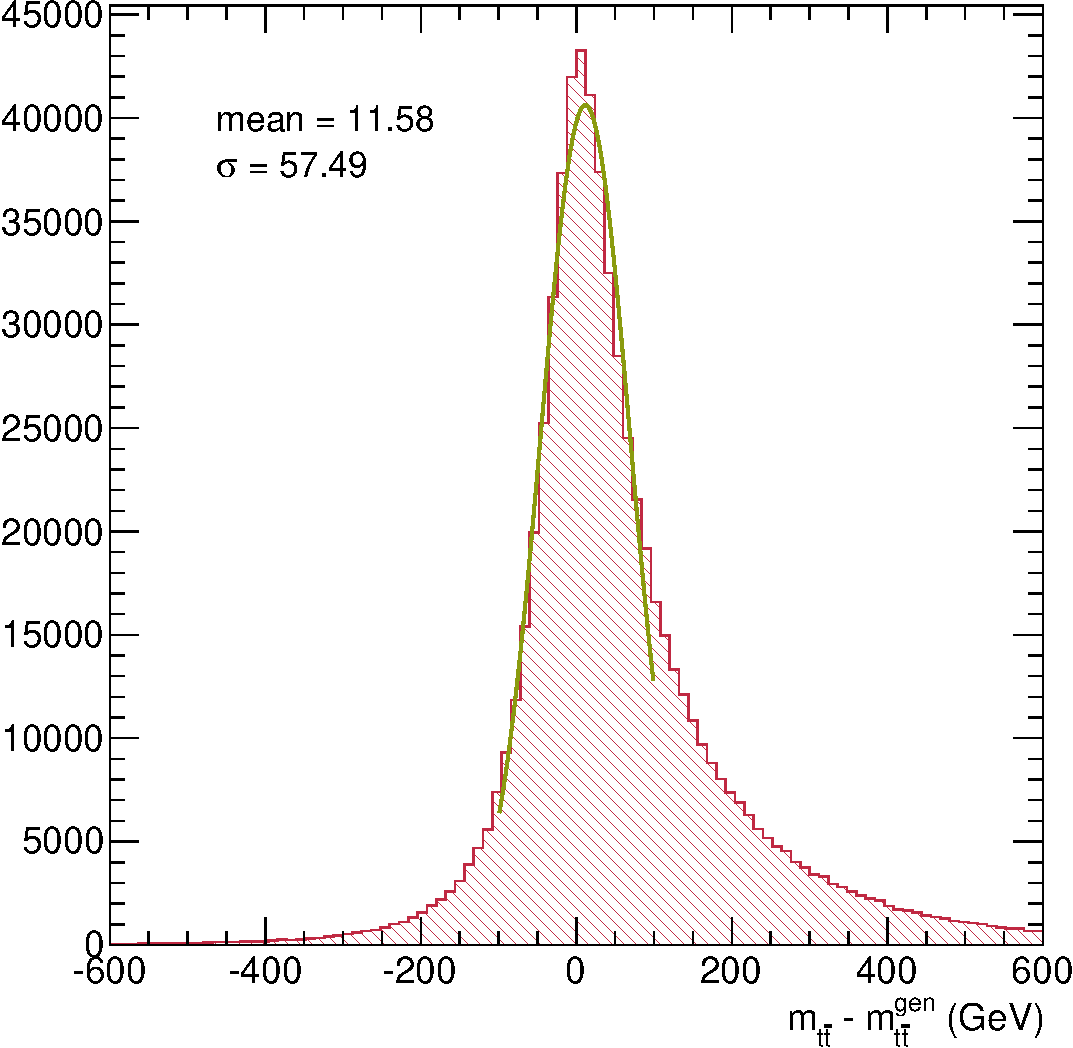
\includegraphics[width=0.48\textwidth]{chapitre6/figs/mtt_resolution_chi2.pdf}} \hfill
    \subcaptionbox{\label{fig:mtt_reso_four_jets}}[0.48\textwidth]{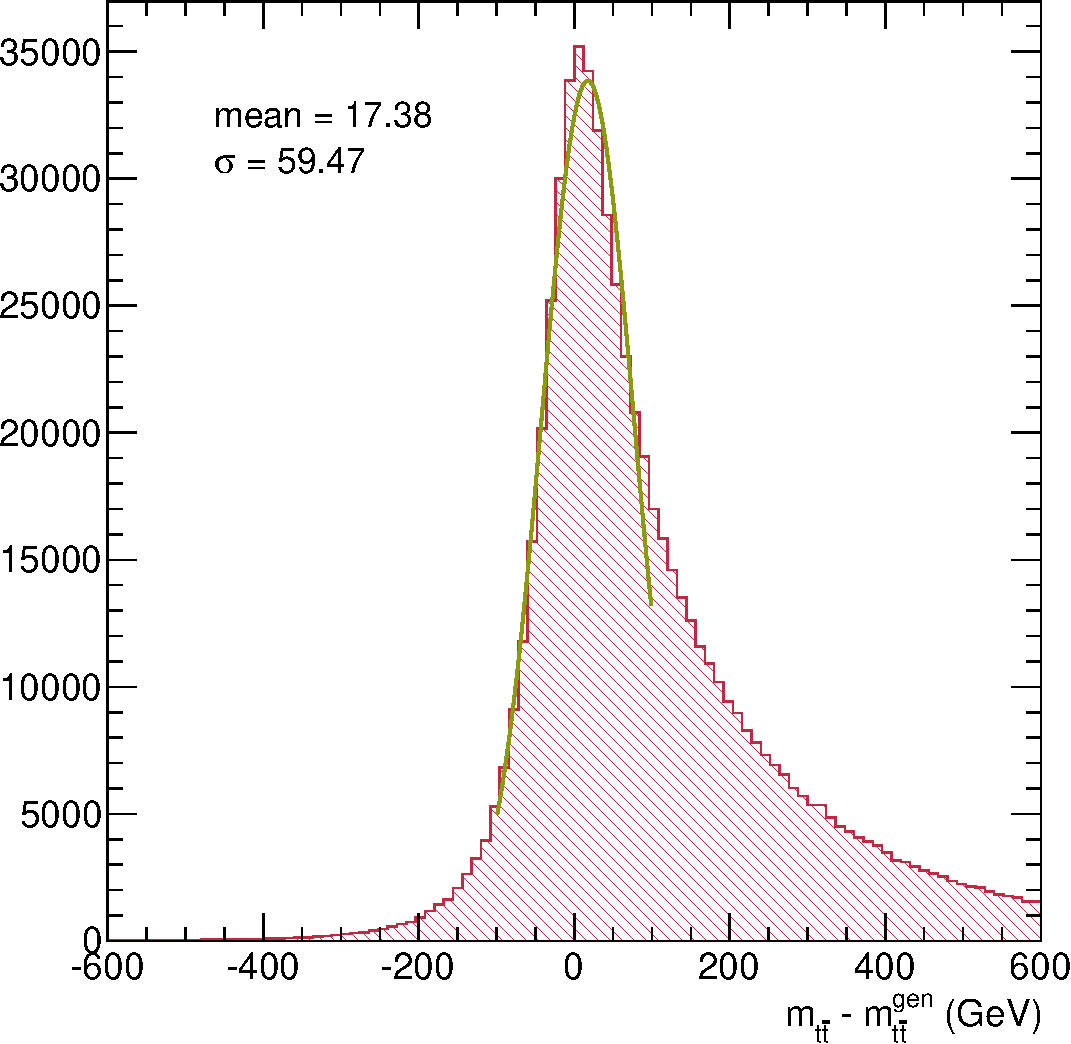
\includegraphics[width=0.48\textwidth]{chapitre6/figs/mtt_resolution_four_jets.pdf}}
    \caption{Résolution de la masse invariante \mtt évaluée sur des événements \ttbar simulés, en utilisant l'algorithme de tri par $\chi^2$ (\subref{fig:mtt_reso_chi2}) et en utilisant les quatre jet de plus haut \pt (\subref{fig:mtt_reso_four_jets}).}
\end{figure}

\begin{figure}[tbp] \centering
    \subcaptionbox{\label{fig:mtt_response_chi2_vs_four_jets}}[0.48\textwidth]{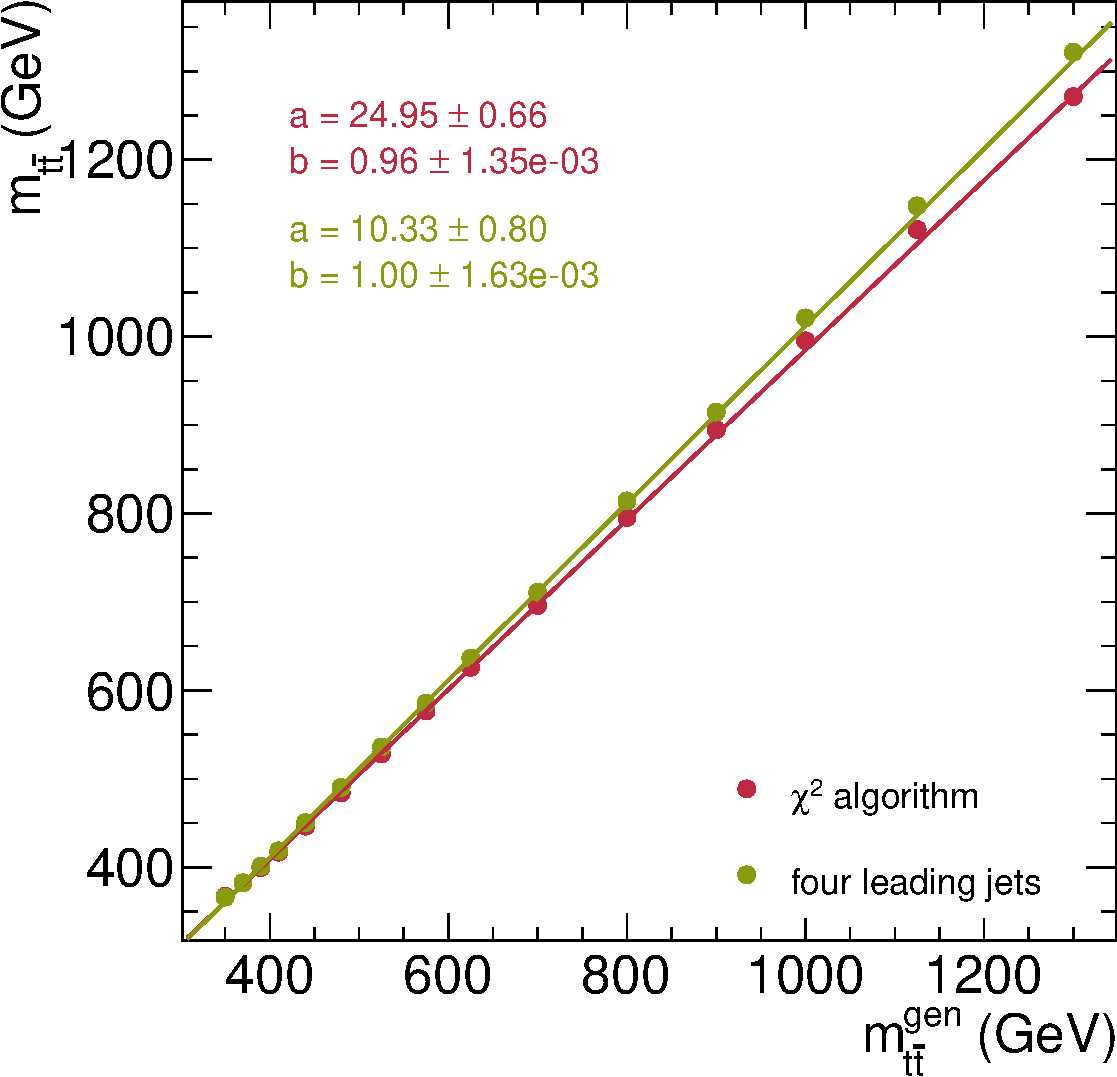
\includegraphics[width=0.48\textwidth]{chapitre6/figs/mtt_response_vs_gen_comparison_chi2_four_jets.pdf}}\hfill
    \subcaptionbox{\label{fig:mtt_reso_vs_mtt_gen_chi2_vs_four_jets}}[0.48\textwidth]{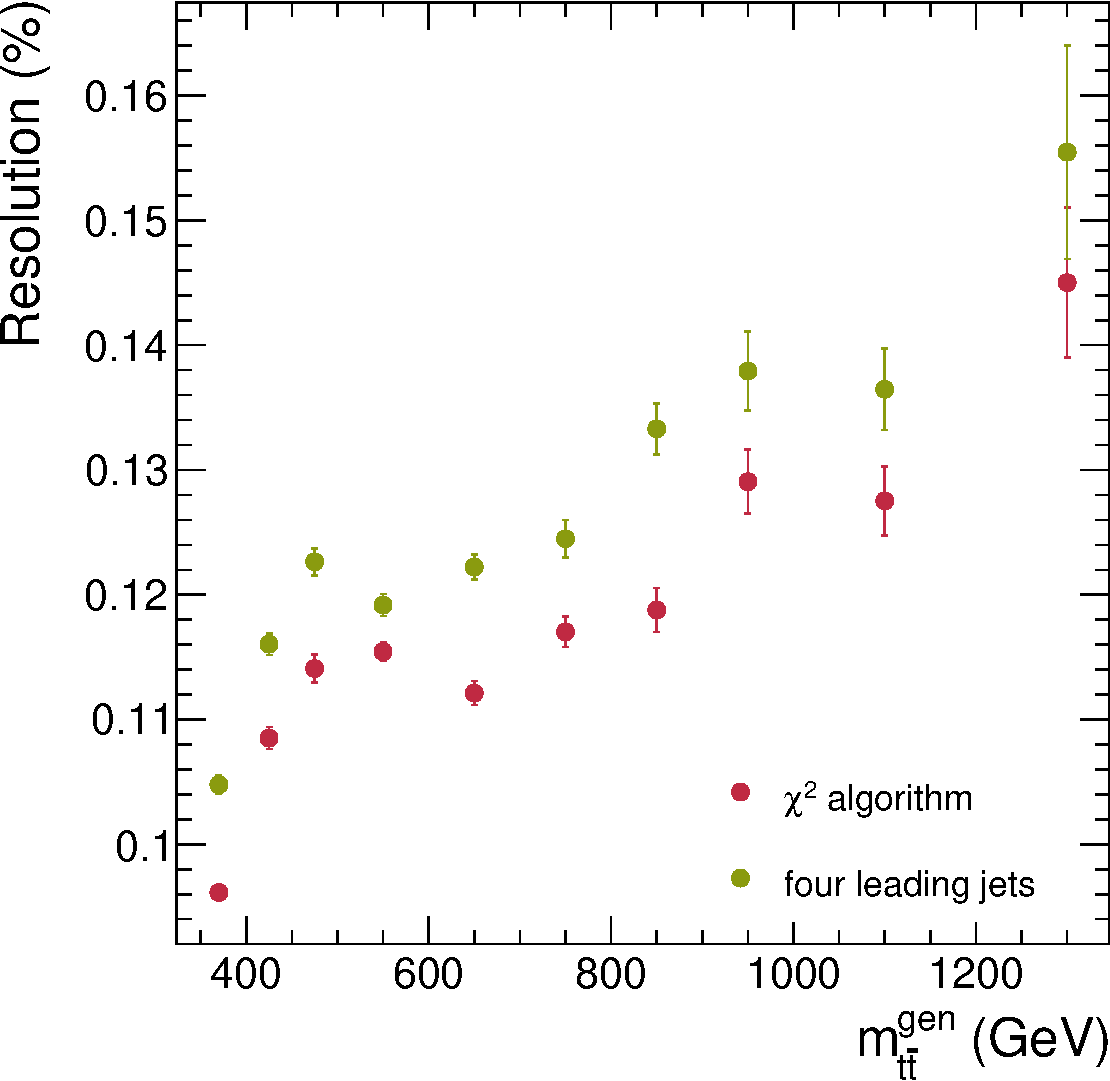
\includegraphics[width=0.48\textwidth]{chapitre6/figs/mtt_resolution_vs_gen_comparison_chi2_four_jets.pdf}}
    \caption{Linéarité de la reconstruction (\subref{fig:mtt_response_chi2_vs_four_jets}) et évolution de la résolution en fonction de $\mtt^\text{gen}$ (\subref{fig:mtt_reso_vs_mtt_gen_chi2_vs_four_jets}) pour l'algorithme de tri par $\chi^2$ (\rouge) et en utilisant les quatre jets de plus haut \pt (\vertc).}
    \label{fig:mtt_reso_chi2_vs_four_jets}
\end{figure}

\bigskip

On compare aussi les performances du BDT par rapport à l'algorithme de tri par $\chi^2$. La \cref{fig:mtt_reso_bdt} présente la résolution sur la masse invariante obtenue avec l'utilisation du BDT (à comparer à la \cref{fig:mtt_reso_chi2}). Là encore, la résolution est dégradée par l'utilisation du BDT. La \cref{fig:mtt_reso_chi2_vs_bdt} confirme cette analyse : la linéarité de la reconstruction est identique entre les deux algorithmes, mais la résolution est dégradée sur toute la gamme de masse invariante.

\begin{figure}[tbp]
  \centering
  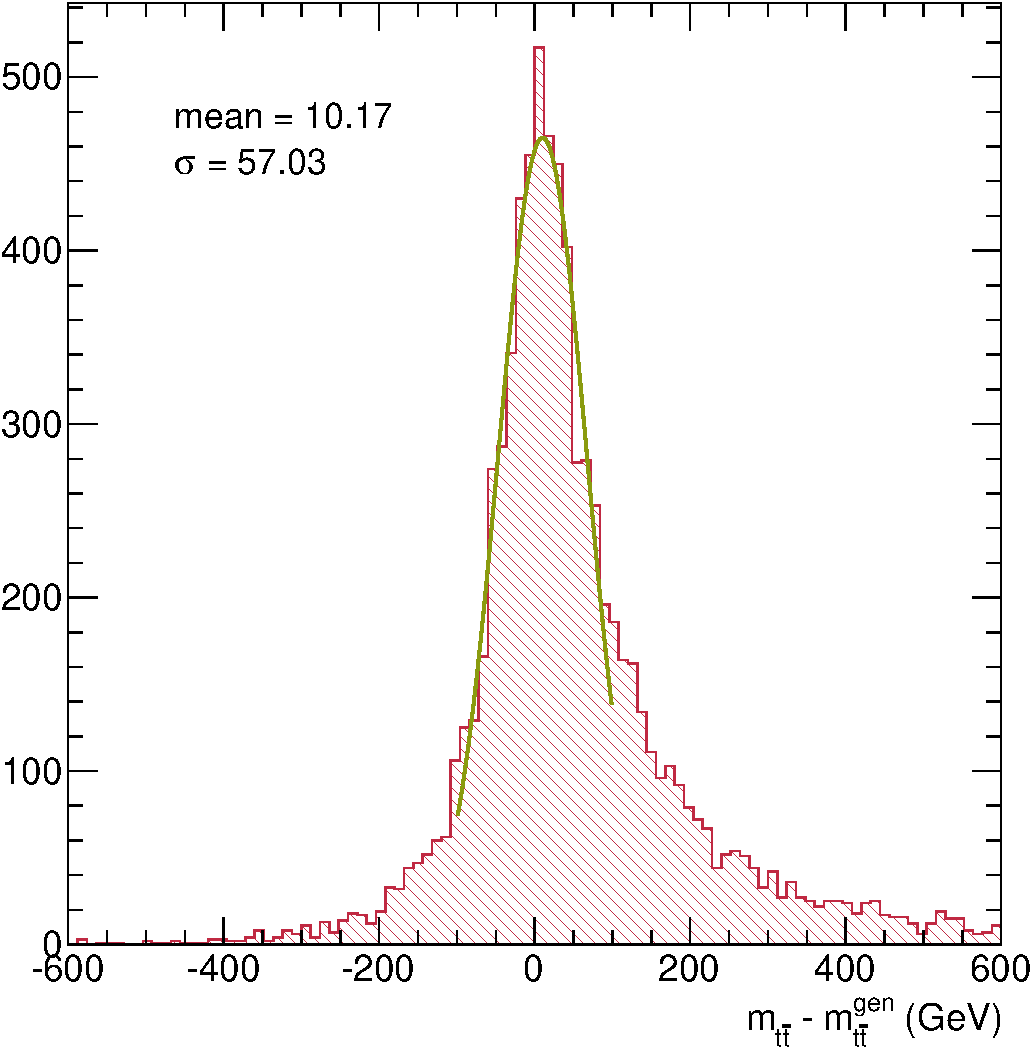
\includegraphics[width=0.48\textwidth]{chapitre6/figs/mtt_resolution_bdt.pdf}
  \caption{Résolution de la masse invariante \mtt obtenue avec l'utilisation du BDT, évaluée sur des événements \ttbar simulés.}
  \label{fig:mtt_reso_bdt}
\end{figure}


\begin{figure}[tbp] \centering
    \subcaptionbox{\label{fig:mtt_response_chi2_vs_bdt}}[0.48\textwidth]{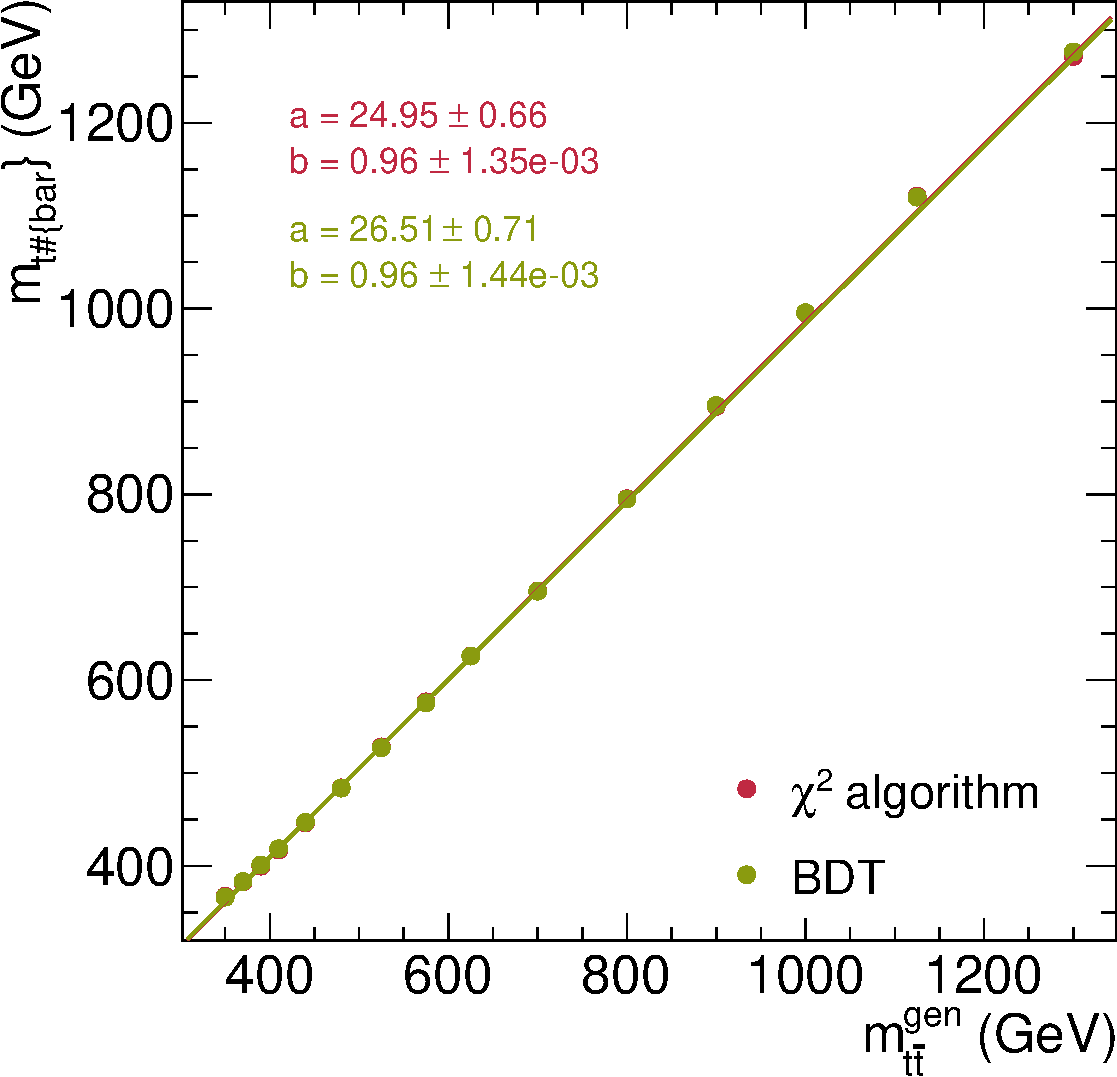
\includegraphics[width=0.48\textwidth]{chapitre6/figs/mtt_response_vs_gen_comparison_chi2_bdt.pdf}}\hfill
    \subcaptionbox{\label{fig:mtt_reso_vs_mtt_gen_chi2_vs_bdt}}[0.48\textwidth]{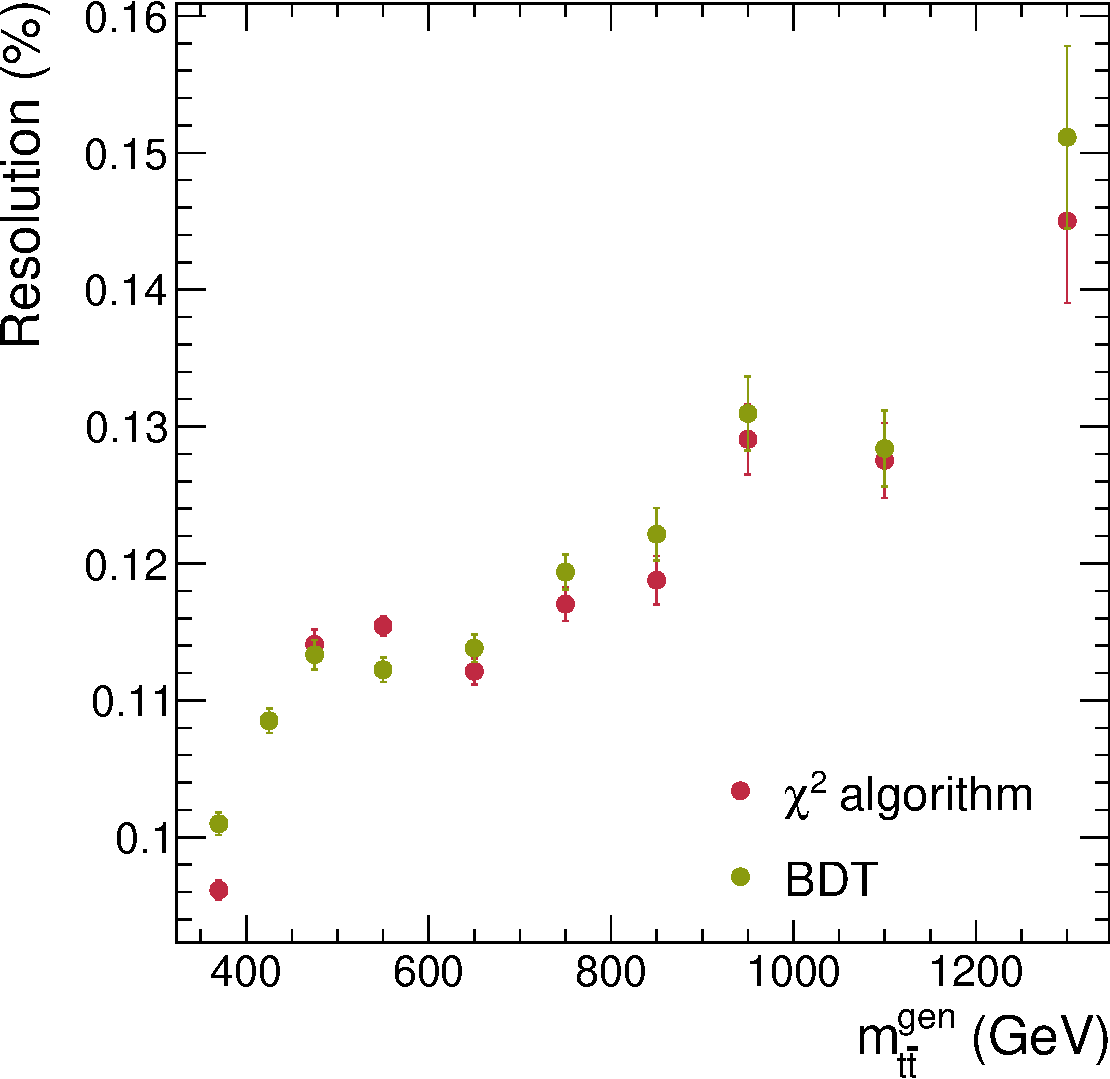
\includegraphics[width=0.48\textwidth]{chapitre6/figs/mtt_resolution_vs_gen_comparison_chi2_bdt.pdf}}
    \caption{Linéarité de la reconstruction (\subref{fig:mtt_response_chi2_vs_bdt}) et évolution de la résolution en fonction de $\mtt^\text{gen}$ (\subref{fig:mtt_reso_vs_mtt_gen_chi2_vs_bdt}) pour l'algorithme de tri par $\chi^2$ (\rouge) et pour le BDT (\vertc).}
    \label{fig:mtt_reso_chi2_vs_bdt}
\end{figure}

\bigskip

Les résultats de cette étude montrent tous que l'algorithme de tri par $\chi^2$ est le plus performant en terme de résolution, au détriment d'une légère perte de linéarité de la reconstruction en fonction de masse invariante générée. Il est intéressant de voir s'il est possible d'améliorer encore les performances de reconstruction en améliorant la résolution. On a en effet vu plus haut qu'une résonance étroite augmente le potentiel de découverte. Un moyen d'améliorer cette résolution est d'utiliser un ajustement cinétique, détaillé dans la suite.

\subsection{Ajustement cinématique} \label{sec:mtt_kf}

Pour un événement \ttbar, les objets reconstruits (leptons, jets, ...) doivent vérifier certaines contraintes cinématiques, telles que la conservation de l'énergie ou reproduire les masses invariantes des particules. Néanmoins, l'impulsion et l'énergie des particules utilisées pour reconstruire l'événement \ttbar ne sont connues qu'avec des incertitudes, liées à la résolution expérimentale, aux techniques de reconstruction, etc. Ces incertitudes peuvent conduire à un non-respect des contraintes d'un événement \ttbar.

\medskip

% L'idée de l'ajustement cinématique est simple : faire varier les quantités physiques des objets sélectionnées, dans leurs incertitudes, afin de respecter au mieux les con\-traintes d'un événement \ttbar. On utilise pour cela la méthode des multiplicateurs de Lagrange afin de trouver les valeurs optimales des quantités physiques des particules sélectionnées sous diverses contraintes.
L'idée de l'ajustement cinématique est simple : on utilise la connaissance de la cinématique d'un événement \ttbar afin d'améliorer la résolution des objets physiques. Les quantités physiques de chaque objet sont optimisées afin de respecter au mieux les contraintes d'un événement \ttbar.

\bigskip

\begin{figure}[p] \centering
    \subcaptionbox{\label{fig:kinfit_matched_events}}[0.48\textwidth]{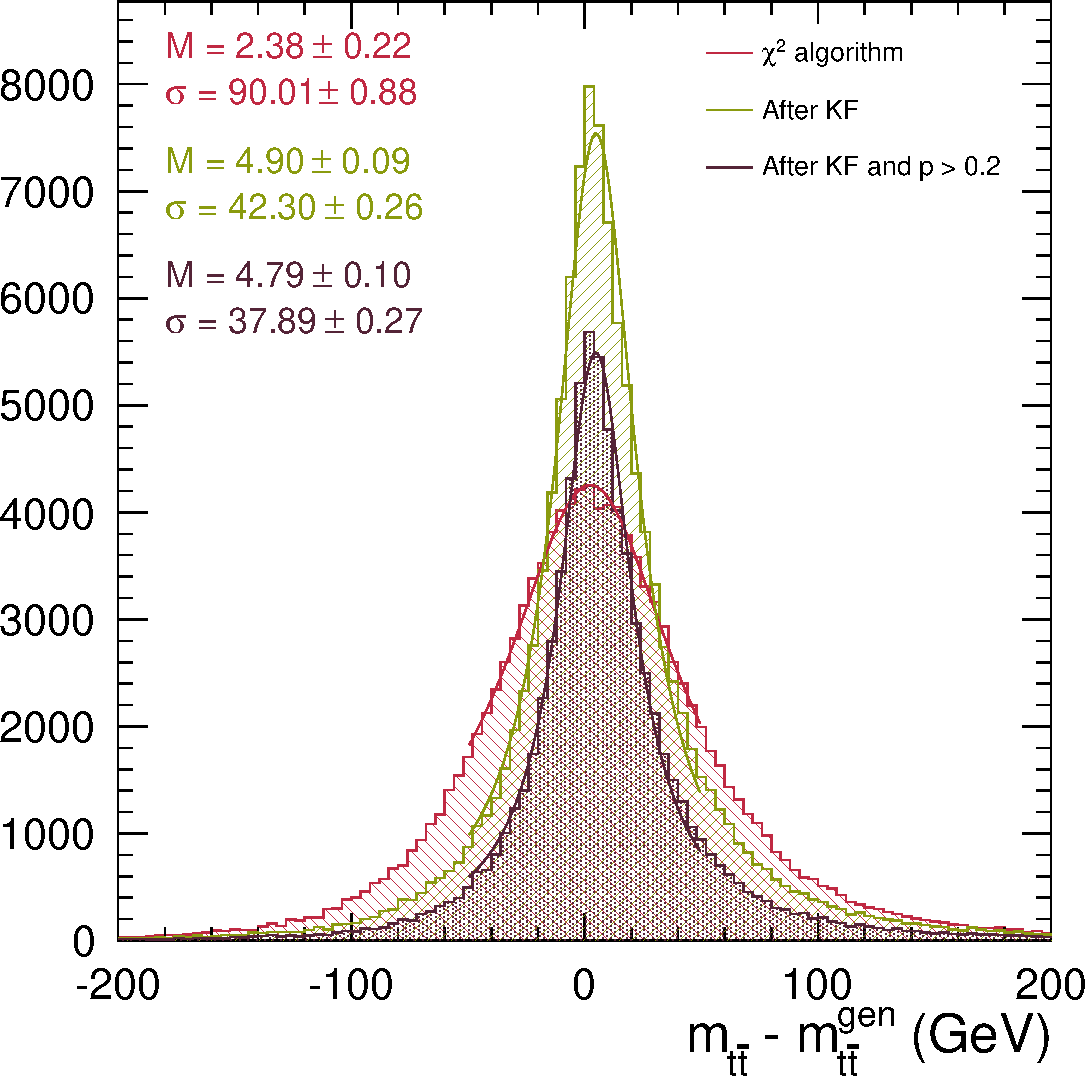
\includegraphics[width=0.48\textwidth]{chapitre6/figs/kinfit/mtt_resolution_comparison_kf_good_solutions.pdf}} \hfill
    \subcaptionbox{\label{fig:kinfit_all_events}}[0.48\textwidth]{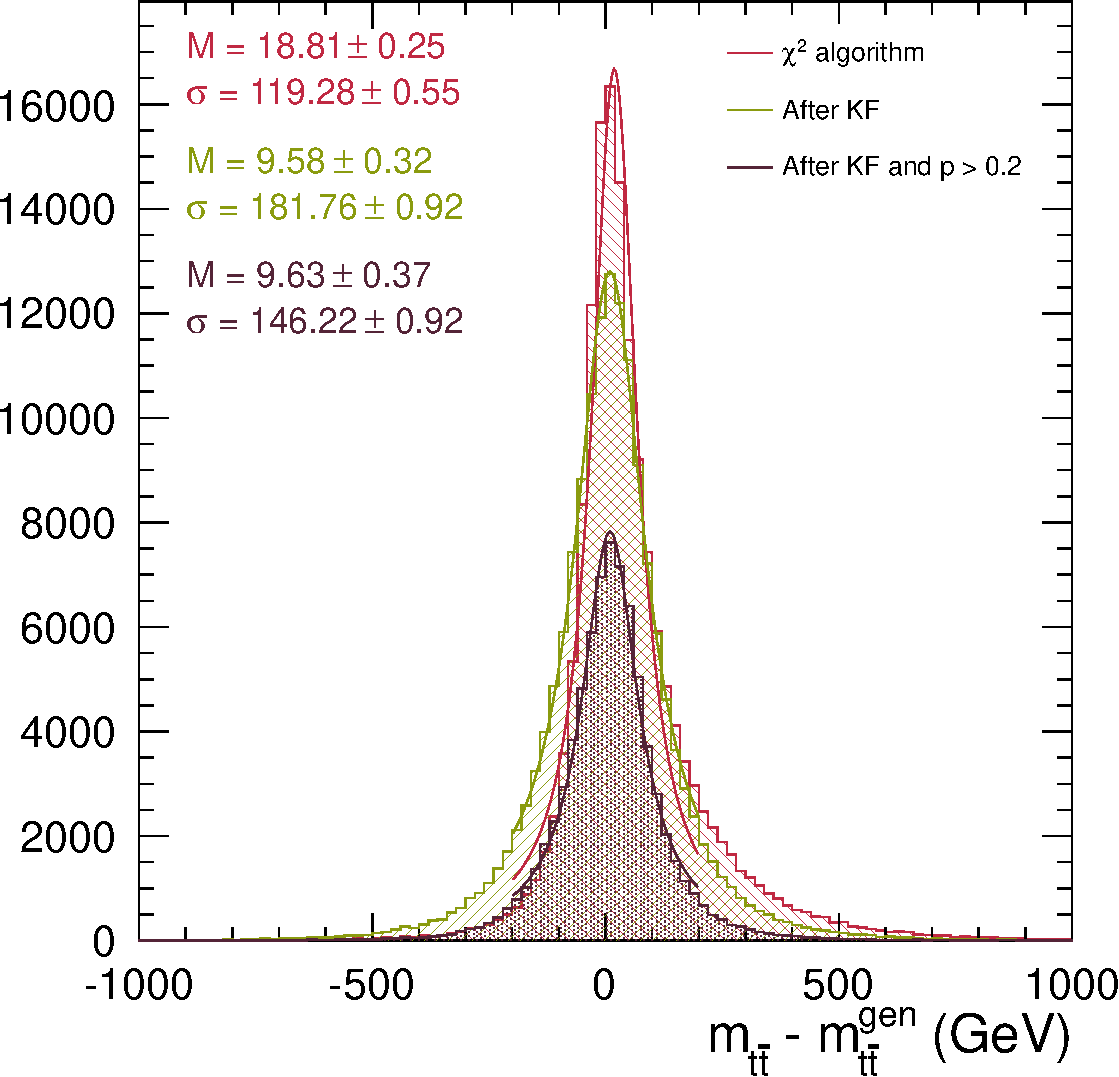
\includegraphics[width=0.48\textwidth]{chapitre6/figs/kinfit/mtt_resolution_comparison_kf_all_events.pdf}}
    \caption{Résolution sur la masse invariante \mtt sans ajustement cinématique (\rouge), après ajustement cinématique (\textcolor{vert}{vert}) et après ajustement cinématique et une coupure $p > \num{0.2}$ (\textcolor{violet}{violet}). Les distributions ont été obtenues avec des événements \ttbar simulés, en utilisant la bonne combinaison de jets (\subref{fig:kinfit_matched_events}) et avec tous les événements (\subref{fig:kinfit_all_events}). Un ajustement avec une Breit-Wigner est superposé afin de facile la comparaison entre les trois méthodes.}
    \label{fig:kinfit_ttbar}
\end{figure}

On utilise l'ajustement cinématique en sortie de l'algorithme de tri par $\chi^2$ : les particules provenant de la désintégration des paires \ttbar sont déjà sélectionnées. L'ajustement cinématique est utilisé pour ajuster au mieux les contraintes, et placer correctement les jets sélectionnés à la bonne position. Les contraintes utilisées dans l'algorithme sont les suivantes :
\begin{itemize}
    \item La masse invariante des deux jets légers doit être égale à la masse du boson \PW.
    \item La masse invariante du neutrino, du lepton ainsi que du jet \Pbottom leptonique doit être égale à la masse du quark top.
    \item La masse invariante des deux jets légers ainsi que du jet \Pbottom hadronique doit être égale à la masse du quark top.
\end{itemize}

% L'effet de l'ajustement cinématique sur la résolution de la masse invariante est présenté \cref{fig:kinfit_ttbar} pour des événements \ttbar simulés. Afin d'améliorer les performances de l'ajustement cinématique, une coupure supplémentaire est réalisée sur la valeur de sortie $p$ de l'algorithme, qui définie la qualité de l'ajustement. On demande $p > 0.2$ (courbe \textcolor{rouge_grandmere}{rouge} sur les distributions des figures \ref{fig:kinfit_ttbar}).

Afin de quantifier les améliorations apportées par l'ajustement cinétique, on présente \cref{fig:kinfit_ttbar} la résolution sur la masse invariante mesurée sur des événements \ttbar simulés. Afin d'améliorer les performances de l'ajustement cinématique, une coupure supplémentaire est réalisée sur la valeur de sortie $p$ de l'algorithme, qui définie la qualité de l'ajustement. On demande $p > \num{0.2}$. On évalue dans un premier temps les performances de l'ajustement sur des événements où la bonne combinaison de jets est sélectionnée par l'algorithme de tri par $\chi^2$. La \cref{fig:mtt_resp_reso_kf_good} présente la linéarité de la reconstruction et l'évolution de la résolution en fonction de la masse invariante \ttbar générée, avant et après utilisation de l'ajustement cinématique. Premièrement, la linéarité est rétablie après l'utilisation de l'ajustement cinématique. De plus, on constate une nette amélioration de la résolution, avec des gains allant de \tilde\SI{75}{\%} à bas \mtt à \tilde\SI{38}{\%} à haut \mtt. La coupure $p > \num{0.2}$ permet de gagner \tilde\SI{10}{\%} à haut \mtt, au détriment d'une diminution du nombre d'événements sélectionnés d'environ \SI{35}{\%}.

\begin{figure}[tbp] \centering
    \subcaptionbox{\label{fig:mtt_response_kf_good}}[0.48\textwidth]{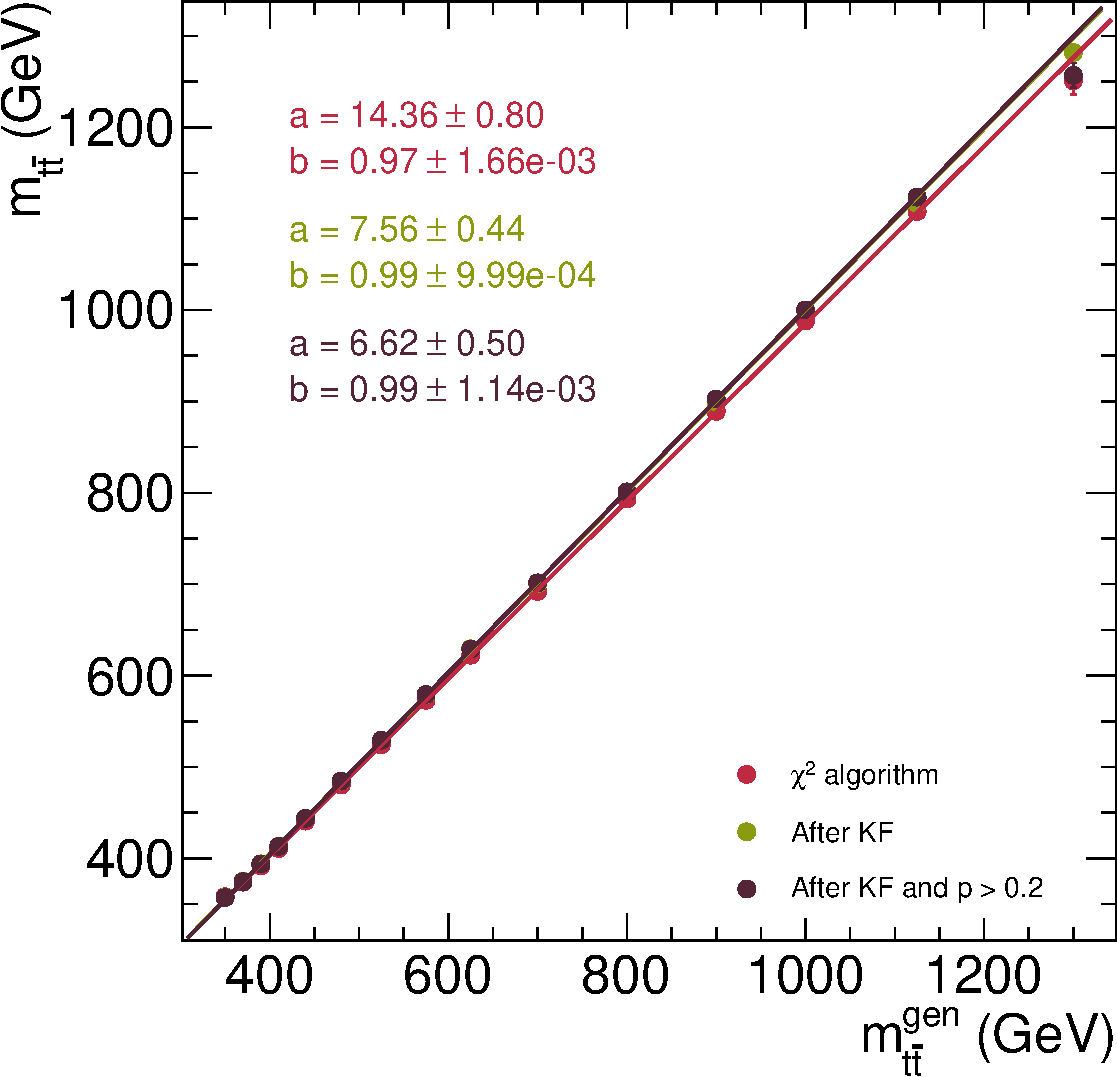
\includegraphics[width=0.48\textwidth]{chapitre6/figs/kinfit/mtt_response_vs_gen_comparison_kf_good_solutions.pdf}} \hfill
    \subcaptionbox{\label{fig:mtt_reso_vs_mtt_gen_kf_good}}[0.48\textwidth]{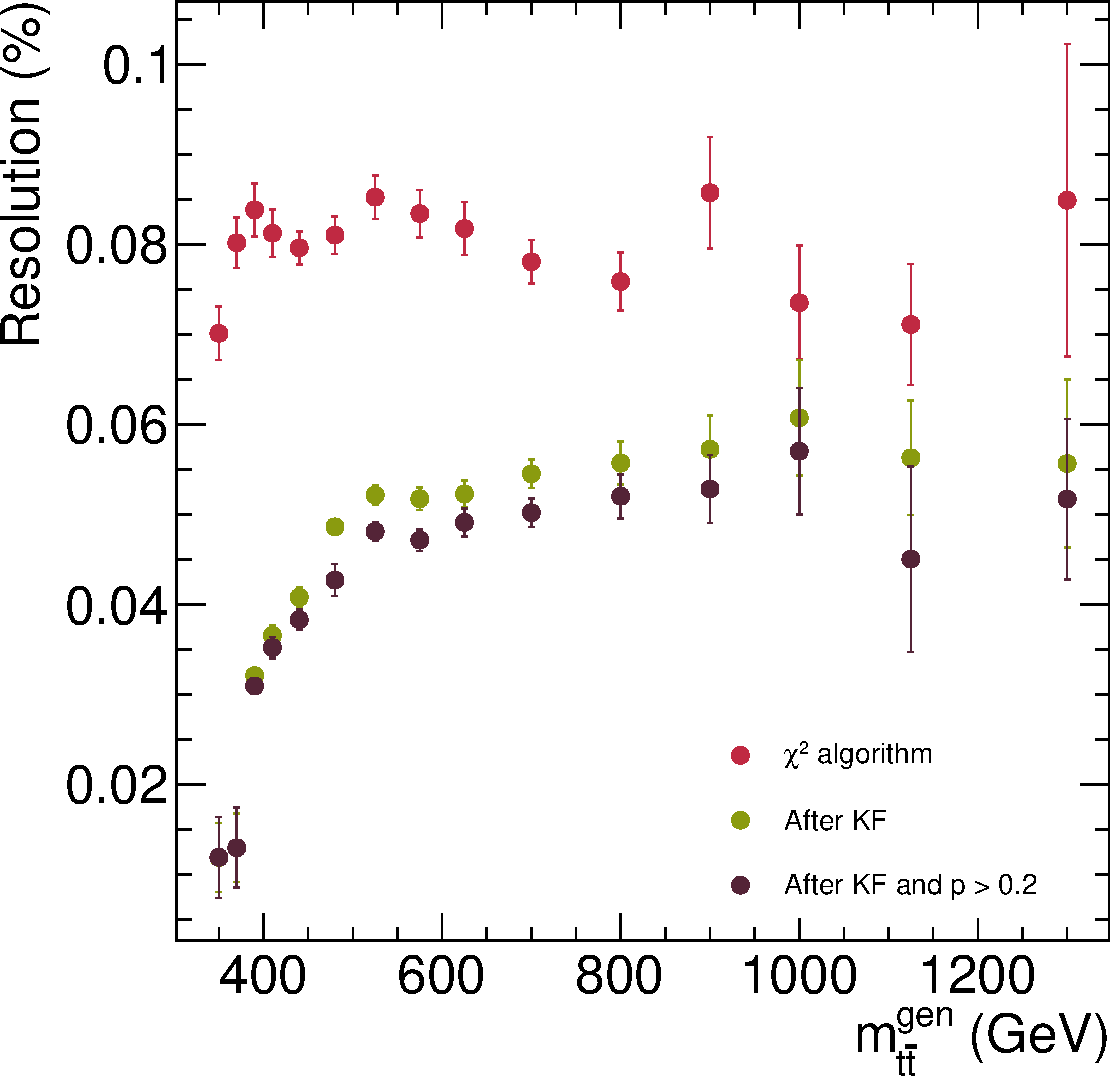
\includegraphics[width=0.48\textwidth]{chapitre6/figs/kinfit/mtt_resolution_vs_gen_comparison_kf_good_solutions.pdf}}
    \caption{Linéarité de la reconstruction (\subref{fig:mtt_response_kf_good}) et évolution de la résolution en fonction de $\mtt^\text{gen}$ (\subref{fig:mtt_reso_vs_mtt_gen_kf_good}) en utilisant la bonne combinaison de jets (\rouge), après utilisation de l'ajustement cinématique (\vertc) et après utilisation de l'ajustement cinématique et $p > \num{0.2}$ (\violet).}
    \label{fig:mtt_resp_reso_kf_good}
\end{figure}

Intéressons nous maintenant aux cas où l'on utilise l'ajustement cinématique sur tous les événements sélectionnés par l'algorithme de tri par $\chi^2$. La \cref{fig:kinfit_all_events} présente la résolution sur la masse invariante, et la \cref{fig:mtt_resp_reso_kf_all_events} la linéarité de la reconstruction ainsi que l'évolution de la résolution en fonction de \mttgen. On note une nette dégradation de la résolution, allant de \tilde\SI{15}{\%} à bas \mtt à \tilde\SI{50}{\%} à haut \mtt. La linéarité de la reconstruction est aussi impactée. On a vu précédemment que l'efficacité d'avoir un événement associable est d'environ \SI{40}{\%} (voir \cref{tab:chi2_study}). Parmi ces événements, l'algorithme de tri par $\chi^2$ choisit environ \num{80} fois sur cent la bonne combinaison de jets : l'ajustement cinématique est donc en mesure de sélectionner la bonne combinaison de jets dans environ \SI{32}{\%} des cas. S'il est très efficace dès lors qu'il utilise la bonne combinaison de jets (voir paragraphe précédent), il dégrade fortement la résolution lorsqu'une mauvaise combinaison est utilisée. Étant donné que des mauvaises combinaisons sont majoritairement sélectionnées, l'utilisation de l'ajustement cinématique dégrade la résolution au lieu de l'améliorer.

\begin{figure}[tbp] \centering
    \subcaptionbox{\label{fig:mtt_response_kf_all}}[0.48\textwidth]{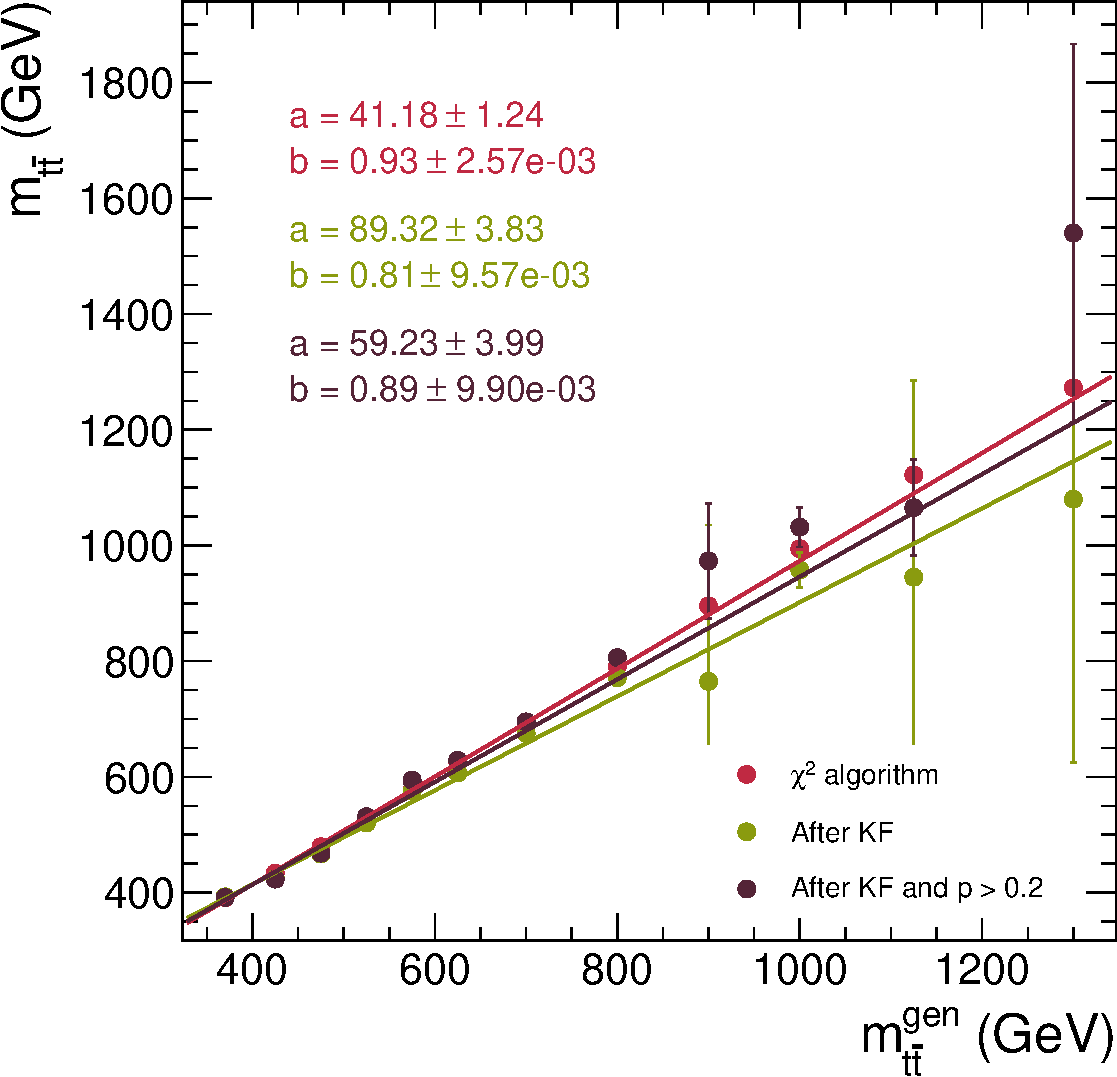
\includegraphics[width=0.48\textwidth]{chapitre6/figs/kinfit/mtt_response_vs_gen_comparison_kf_all_events.pdf}} \hfill
    \subcaptionbox{\label{fig:mtt_reso_vs_mtt_gen_kf_all}}[0.48\textwidth]{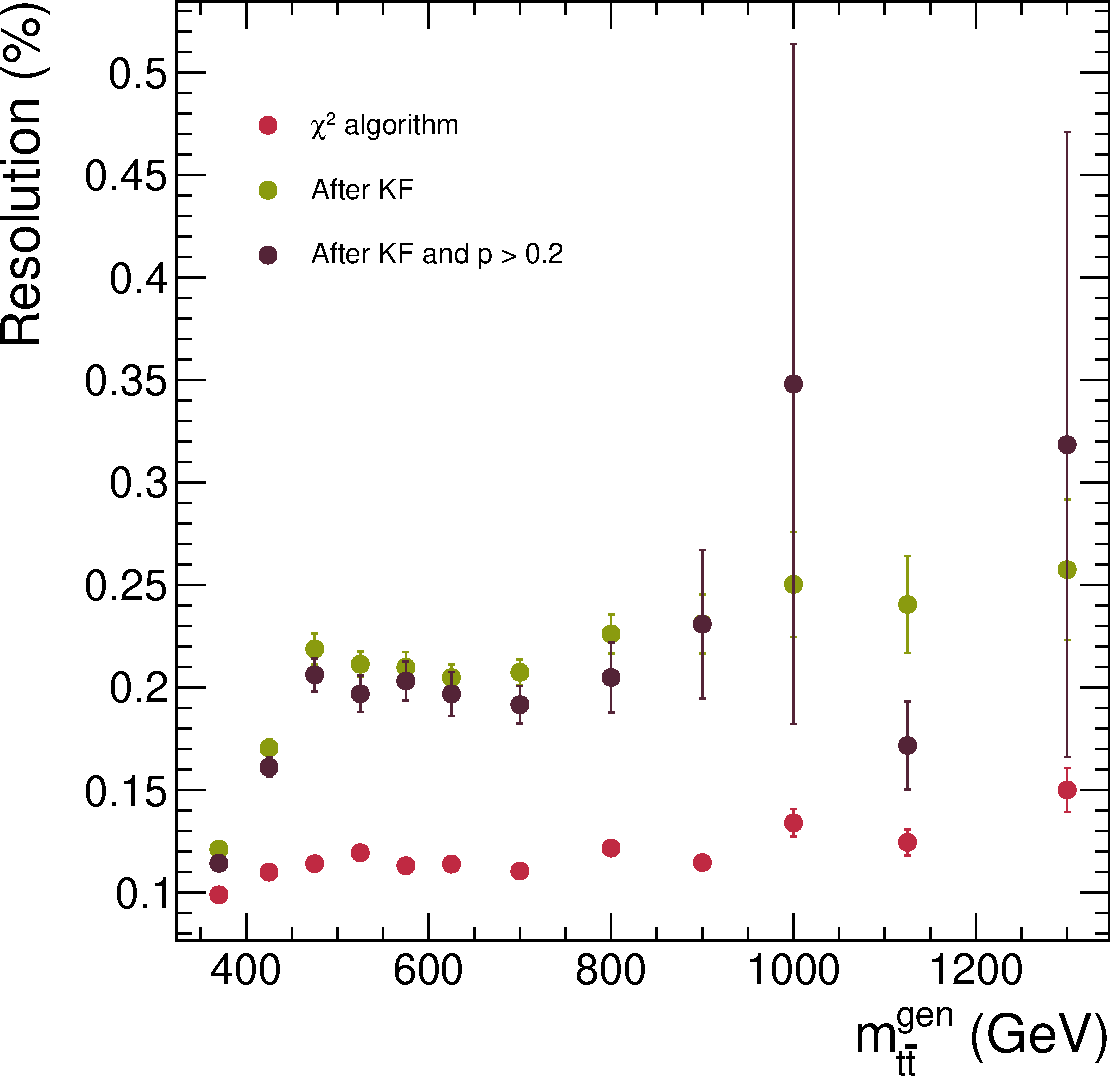
\includegraphics[width=0.48\textwidth]{chapitre6/figs/kinfit/mtt_resolution_vs_gen_comparison_kf_all_events.pdf}}
    \caption{Linéarité de la reconstruction (\subref{fig:mtt_response_kf_all}) et évolution de la résolution en fonction de $\mtt^\text{gen}$ (\subref{fig:mtt_reso_vs_mtt_gen_kf_all}) en utilisant les jets sélectionnés par l'algorithme de $\chi^2$ (\rouge), après utilisation de l'ajustement cinématique (\vertc) et après utilisation de l'ajustement cinématique et $p > \num{0.2}$ (\violet).}
    \label{fig:mtt_resp_reso_kf_all_events}
\end{figure}

\bigskip

On verra dans le \cref{chap:zprime} que ces résultats, obtenus sur des événements \ttbar du Modèle Standard, sont généralisables aux événements \ttbar produit par de la nouvelle physique. La résolution obtenue au final est fortement dégradée par l'utilisation de l'ajustement cinématique, ce qui nous a poussé à ne pas l'utiliser pour reconstruire la masse invariante \ttbar.

%On verra dans le \cref{chap:zprime} que ces bons résultats sur des événements \ttbar du Modèle Standard n'impliquent pas forcément de bonnes performances pour des événements \ttbar produits par de la nouvelle physique. En effet, l'ajustement cinématique est optimiser pour la cinématique de la désintégration de paires \ttbar Modèle Standard, et on verra dans le prochain chapitre que cette cinématique peut être vraiment différente dans le cas de nouvelle physique. À cause de cette différence, on observe une dégradation de la résolution lors de l'utilisation de l'ajustement cinématique. Cette dégradation nous a poussé à ne pas utiliser l'ajustement cinématique pour reconstruire la masse invariante \ttbar.

\section{Conclusion}

Comme on a pu le voir tout au long de ce chapitre, deux étapes sont nécessaires pour reconstruire la masse invariante \ttbar. Dans un premier temps, il est nécessaire de choisir correctement les jets provenant de la désintégration des quarks top, et non pas des jets provenant du \pu ou de radiations. On utilise pour cela un algorithme de tri par $\chi^2$, qui s'est trouvé plus performant que des algorithmes plus complexes comme les MVA. Une fois les jets sélectionnés, il reste à reconstruire la composante longitudinale de l'impulsion du neutrino, ce qui permet d'évaluer correctement l'énergie. Finalement, il est possible de reconstruire la masse invariante du système \ttbar. La résolution typique obtenue sur cette reconstruction est d'environ \SI{10}{\percent}.

\bigskip

Toutes ces techniques sont utilisées dans les analyses de recherche de nouvelles physiques, comme on le verra dans les \cref{chap:zprime,chap:higgs}.